% ============================================================
%  EDCI 59100-016  |  Assignment 11: Final Literature Review Manuscript
%  Md Kamruzzaman Kamrul  |  Summer 2026
% ============================================================
\documentclass[10pt,letterpaper]{article}

\usepackage[margin=0.75in, top=0.85in, bottom=0.85in]{geometry}
\usepackage{array}
\usepackage{booktabs}
\usepackage{longtable}
\usepackage{tabularx}
\usepackage{pdflscape}
\usepackage[table]{xcolor}
\usepackage{titlesec}
\usepackage{fancyhdr}
\usepackage{enumitem}
\usepackage{microtype}
\usepackage[hidelinks]{hyperref}
\usepackage{tikz}
\usepackage{pgfplots}
\pgfplotsset{compat=1.17}
\usepackage{pgf-pie}
\usetikzlibrary{shapes.geometric, arrows.meta, positioning, fit, calc}
\usepackage{setspace}
\usepackage{caption}
\usepackage{subcaption}
\usepackage{float}
\usepackage{amsmath}
\usepackage{graphicx}
\usepackage{multirow}

\definecolor{headingblue}{HTML}{1F4E79}
\definecolor{lightblue}{HTML}{D9EAF7}
\definecolor{softgray}{HTML}{F4F6F8}
\definecolor{darkgray}{HTML}{404040}
\definecolor{prismagreen}{HTML}{E8F5E9}
\definecolor{prismabox}{HTML}{1565C0}
\definecolor{chartblue}{HTML}{2196F3}
\definecolor{chartorange}{HTML}{FF9800}
\definecolor{chartgreen}{HTML}{4CAF50}
\definecolor{chartred}{HTML}{F44336}
\definecolor{chartpurple}{HTML}{9C27B0}
\definecolor{chartgray}{HTML}{9E9E9E}

\pagestyle{fancy}
\fancyhf{}
\lhead{\small Md Kamruzzaman Kamrul}
\chead{\small EDCI 59100-016 \textbar{} Final Literature Review Manuscript}
\rhead{\small Summer 2026}
\cfoot{\small \thepage}
\renewcommand{\headrulewidth}{0.4pt}
\setlength{\headheight}{14pt}

\titleformat{\section}{\normalfont\large\bfseries\color{headingblue}}{\thesection.}{0.5em}{}
\titleformat{\subsection}{\normalfont\normalsize\bfseries\color{headingblue}}{\thesubsection.}{0.5em}{}
\titleformat{\subsubsection}{\normalfont\normalsize\bfseries\color{darkgray}}{\thesubsubsection.}{0.45em}{}
\titlespacing*{\section}{0pt}{11pt}{4pt}
\titlespacing*{\subsection}{0pt}{8pt}{3pt}
\titlespacing*{\subsubsection}{0pt}{6pt}{2pt}

\setlength{\parindent}{0pt}
\setlength{\parskip}{5pt}
\setlist[itemize]{leftmargin=*,itemsep=2pt,topsep=2pt}
\setlist[enumerate]{leftmargin=*,itemsep=2pt,topsep=2pt}
\renewcommand{\arraystretch}{1.18}
\setlength{\tabcolsep}{4pt}
\emergencystretch=3em

\newcolumntype{L}[1]{>{\raggedright\arraybackslash}p{#1}}
\newcolumntype{Y}{>{\raggedright\arraybackslash}X}

\captionsetup{font=small, labelfont=bf}

% ============================================================
\begin{document}

\begin{center}
{\Large\bfseries\color{headingblue} Vision-Language Models for Construction Site Safety and Progress Monitoring: A Scoping Review}\\[0.5em]
{\normalsize Md Kamruzzaman Kamrul}\\[0.15em]
{\small Lyles School of Civil and Construction Engineering, Purdue University, West Lafayette, IN, USA}\\[0.15em]
{\small Corresponding author: \href{mailto:mkamrul@purdue.edu}{mkamrul@purdue.edu}}\\[0.2em]
{\small EDCI 59100-016 \textbar{} Summer 2026 \textbar{} Final Literature Review Manuscript (Assignment 11)}\\[0.15em]
{\small Discipline: Civil Engineering / Construction Management \textbar{} Format: Numbered citation style consistent with \textit{Automation in Construction} (Elsevier)}
\end{center}

\vspace{0.3em}

% ---------- Abstract ----------
\begin{center}
\begin{minipage}{0.93\textwidth}
{\color{headingblue}\bfseries\small ABSTRACT}\\[0.3em]
{\small
Construction sites are dynamic, safety-critical environments where managers must simultaneously prevent hazards and track production. Manual monitoring is slow, subjective, and error-prone, while prior automation has been split between computer vision, which perceives the site but cannot reason over regulations, and natural language processing, which encodes rules but cannot see. Vision-language models (VLMs) promise to close this gap by jointly processing visual and textual data, yet their application to construction has not been systematically mapped. This paper presents a scoping review, conducted following the PRISMA-ScR guidelines, of VLM and multimodal artificial-intelligence applications for construction site safety and progress monitoring. Searches of Web of Science and Scopus, complemented by backward snowballing, yielded a final corpus of 58 peer-reviewed studies (2009--2026). Using a thematic synthesis organized by a three-layered framework (sensory inputs, cognitive engine, construction outputs), the review identifies three architectural paradigms: zero/few-shot retrieval, domain fine-tuned generative captioning, and hybrid agentic systems. These paradigms coexist rather than supersede one another, and progress tracking---not safety---is the dominant application across all three. The review surfaces four field-level gaps: fragmented evaluation with no shared benchmark, near-universal reliance on private datasets (79\% of core studies), underdeveloped temporal reasoning, and a systematic absence of real-site validation. To the authors' knowledge, this is the first PRISMA-ScR scoping review to map vision-language-model architectural-paradigm evolution across construction safety and progress monitoring, offering a reusable classification framework and an actionable research agenda.
}\\[0.4em]
{\small\textbf{Keywords:} Vision-language models; Multimodal learning; Construction safety; Progress monitoring; Scoping review; Construction scene understanding}
\end{minipage}
\end{center}

\vspace{0.4em}

% ============================================================
\section{Introduction}
% ============================================================

Construction sites are dynamic environments where workers, equipment, and machines operate simultaneously under conditions that make monitoring both necessary and difficult \cite{alaloul2022}. Unlike aerospace or automotive manufacturing, construction is labor-intensive, project-specific, and organized around ad-hoc supply chains. These characteristics render standard industrial monitoring systems impractical \cite{davila2021,alaloul2022}.

Site managers carry two parallel responsibilities: keeping the environment hazard-free through regular safety inspection \cite{asadzadeh2020}, and tracking activity progress against production targets \cite{alaloul2022}. Both tasks rely on manual observation---physical walk-throughs, visual hazard checks, and hand-logged Daily Construction Reports (DCRs)---which is subjective, error-prone, and slow \cite{samsami2024}. Progress monitoring is especially exposed: because production status is inferred from intermittent manual reports, the resulting information lag impairs schedule and cost control and limits managers' ability to detect variability before it compounds \cite{sherafat2020}.

These bottlenecks explain the industry's persistent safety and productivity challenges \cite{jiang2023}, and have driven growing adoption of AI---particularly computer vision---as an automated alternative \cite{rabbi2024,paneru2021}.

To overcome the data deficiencies of traditional manual methods, research initially shifted toward automated object-level data collection \cite{tuomisto2026}. Rather than broadly applying automation to all construction tasks, this specific technological domain focused on developing automated, real-time performance monitoring systems consisting of location tracking, activity recognition, and performance monitoring \cite{sherafat2020}. To achieve this, the first of these methods involved attaching tracking devices like Radio Frequency Identification (RFID), Ultra-Wideband (UWB), or Bluetooth Low Energy (BLE) to building components \cite{asadzadeh2020}. However, while these tag-based methods are effective for locating materials, they cannot verify the proper installation or condition of components, limiting their utility for detailed inspection tasks \cite{sherafat2020}. Furthermore, tracking eventually thousands of items does not offer an economical or practical approach in large-scale projects \cite{bohn2010}. The field therefore adopted computer vision techniques. Cameras require no sensor attachments and capture the locations and activities of construction entities, providing both operational and technical advantages over wearable-sensor systems \cite{xiong2019}.

Building upon the shift toward camera-based monitoring, the field widely deployed traditional computer vision approaches utilizing bounding-box detectors to locate construction entities. While these models are highly effective at spatial localization, identifying only the workers and PPE components, without recognizing the contextual relationship between them, does not effectively verify PPE compliance \cite{nath2020}. Specifically, inferring that workers are prone to falling from height based on safety regulations is difficult for computer vision; this condition can be summarized as a \textit{semantic gap}---a long-recognized computer-vision problem applied to the construction compliance context by Wu et al.\ \cite{wu2021}. Because computer vision cannot natively comprehend safety rulebooks, traditional pipelines attempted to bridge this gap by applying an algorithm with explicit rules determined through empirical observations \cite{nath2020}. However, manually establishing these rules for multiple PPEs is a complicated task and results may not be structured or comprehensive enough to consider all possible scenarios \cite{nath2020}.

To overcome the limitation of manual geometric mapping, research explored an alternative approach using Natural Language Processing (NLP) for automatically extracting regulatory requirements from textual regulatory documents and formalizing these requirements in a logic format \cite{zhang2015}. Yet, while NLP excels at rule extraction, these text-based models are fundamentally blind to the physical site. Ultimately, they simply represent the extracted safety requirements in the form of query graphs for supporting subsequent knowledge graph-based field compliance checking \cite{wang2023}. Consequently, this creates a clear technological disconnect: computer vision can see the site but cannot understand the rules, while NLP understands the rules but cannot see the site. This limitation motivates the emergence of multimodal Vision-Language Models (VLMs) capable of natively fusing both data streams.

To address the limitations of traditional methods in processing semantic information, recent advances have introduced models that jointly process pixels and text. We use \textit{vision-language model} (VLM) as the umbrella term for any architecture that aligns visual inputs with natural language in a shared representational space; the terms \textit{multimodal large language model} (MLLM) and \textit{large multimodal model} (LMM) denote the generative, instruction-following subclass of VLMs and are used interchangeably in the source literature. By extracting both visual and linguistic features, these models perform instruction-following tasks such as image captioning, visual grounding, and visual question answering (VQA) \cite{chan2025}. Furthermore, these architectures acquire generalized visual representations guided by natural language supervision, enabling impressive zero-shot detection capabilities \cite{zhang2025}. By leveraging natural language prompts and contextual reasoning, VLMs offer a flexible approach for spatiotemporal analysis. They interpret both the spatial geometry of hazards and the temporal sequence of complex human behaviors on dynamic construction sites, potentially reducing dependence on extensive labeled datasets \cite{bui2026}. Consequently, these multimodal systems can create human-readable captions for daily progress and work activity logs \cite{jung2024}, while simultaneously supporting interactive question-and-answer sessions, fostering a more informed understanding of construction site safety \cite{hussain2026}.

Despite the rapid emergence of VLMs, existing reviews have remained siloed in their respective unimodal domains. Most reviews of AI applications in construction focus on a single technology---computer vision or NLP---thereby addressing only fragments of the potential application space \cite{rabbi2024}. Previous reviews have extensively mapped pure computer vision research in construction \cite{jiang2023,paneru2021,zhong2019}, surveyed sensor-based safety management \cite{asadzadeh2020}, or characterized automated activity and progress monitoring \cite{sherafat2020,samsami2024}. While these studies provide valuable baselines, they predate or only briefly touch the multimodal turn, and none maps VLM architectures at the paradigm level across both safety and progress monitoring \cite{zhang2025}. Although VLMs excel in general multimodal tasks, their ability to interpret human behavior in safety-critical construction environments remains largely unexplored \cite{bui2026}. Table~\ref{tab:priorreviews} situates this review against the most relevant prior reviews, mapping each by primary technology focus, application scope, and whether VLM architectural paradigms were addressed.

\begin{table}[H]
\caption{Positioning of this review relative to prior reviews of AI in construction.}
\label{tab:priorreviews}
\small
\rowcolors{2}{softgray}{white}
\begin{tabularx}{\textwidth}{L{3.5cm} L{3.6cm} Y L{2.3cm}}
\toprule
\rowcolor{lightblue}
\textbf{Review (Year)} & \textbf{Primary technology focus} & \textbf{Application scope} & \textbf{VLM paradigms mapped?}\\
\midrule
Zhong et al.\ (2019) & Computer vision & General CV in construction & No\\
Asadzadeh et al.\ (2020) & Wearable / proximity sensors & Safety management & No\\
Sherafat et al.\ (2020) & Vision + sensor fusion & Worker/equipment activity recognition & No\\
Paneru \& Jeelani (2021) & Computer vision & General CV; opportunities and challenges & No\\
Jiang \& Messner (2023) & Computer vision & CV across asset-management phases & No\\
Rabbi \& Jeelani (2024) & AI (text, vision, audio) & Construction safety & Partial (named, not paradigm-level)\\
Samsami (2024) & Automated CV / progress & Inspection and progress monitoring & No\\
Li et al.\ (2025) & Scene understanding (incl.\ DL/VLM) & Worker-centric safety & Emerging (safety only)\\
\rowcolor{prismagreen}
\textbf{This review (2026)} & \textbf{Vision-language / multimodal} & \textbf{Safety \emph{and} progress monitoring} & \textbf{Yes (paradigms A/B/C)}\\
\bottomrule
\end{tabularx}
\end{table}

As Table~\ref{tab:priorreviews} shows, no prior review maps VLM architectural paradigms across both construction safety and progress monitoring. To address this gap, this paper presents a scoping review of multimodal vision-language systems applied to both domains. Conducted in accordance with the PRISMA-ScR guidelines \cite{tricco2018}, and to the authors' knowledge the first PRISMA-ScR scoping review to map vision-language-model architectural-paradigm evolution across construction safety and progress monitoring, the objectives of this study are to: (1) map the current landscape of VLM applications in construction management; (2) organize the literature using a three-layered synthesis framework that links foundational VLM architectures to practical construction management deliverables; and (3) analyze algorithmic limitations to outline a research agenda. To achieve these objectives, the review answers four research questions (RQs):

\begin{itemize}
  \item \textbf{RQ1:} What are the prevalent Vision-Language Model (VLM) architectures currently utilized for spatiotemporal analysis in construction?
  \item \textbf{RQ2:} How is multimodal data (visual and textual) fused and processed across construction safety and progress monitoring applications?
  \item \textbf{RQ3:} What are the primary methodological bottlenecks in deploying these models for real-time progress tracking and safety?
  \item \textbf{RQ4:} How is the performance of Vision-Language Models currently evaluated and benchmarked across construction safety and progress monitoring tasks?
\end{itemize}

% ============================================================
\section{Research Methodology}
% ============================================================

This review was conducted in accordance with the PRISMA-ScR (Preferred Reporting Items for Systematic Reviews and Meta-Analyses extension for Scoping Reviews) guidelines \cite{tricco2018}. This review adopts a scoping design rather than quantitative meta-analysis for two reasons. First, VLMs represent an emerging architecture whose extent, range, and nature in construction applications requires mapping before any narrow intervention comparison is appropriate \cite{chan2025,chen2024}. Second, the included studies use heterogeneous evaluation metrics: geometric precision measures such as mean Average Precision \cite{nath2020,wang2024} alongside natural language generation metrics such as BLEU and CIDEr \cite{jung2024,xiao2022}. This heterogeneity makes standardized statistical synthesis impossible.

Methodologically, the review employs a mixed-method design. PRISMA-ScR governs the transparent identification, screening, and descriptive mapping of the evidence (Sections~2.1--3), establishing \emph{what} research exists. A thematic synthesis framework then serves as the analytical lens (Section~4), organizing the mapped literature into architectural paradigms to interpret \emph{how} the field is structured. Combining a scoping protocol with a synthesis framework is established practice for reviews of fast-moving, heterogeneous technologies, where a purely descriptive map would under-serve the reader and a full systematic appraisal would be premature \cite{sherafat2020}.

\subsection{Search Strategy and Information Sources}

To ensure a rigorous and reproducible retrieval process, the literature search was conducted on 4\textsuperscript{th} March 2026 across two of the most comprehensive scientific databases for engineering and computer science research: the Web of Science (WoS) Core Collection and Scopus. These specific databases were selected because WoS contains the most comprehensive and influential journals within the field of construction and engineering management \cite{zhong2019}, and Scopus is actively used alongside WoS as a primary search engine for AI applications in the construction domain \cite{rabbi2024}. The keywords were determined by analyzing frequent words found in papers where AI was applied to enhance construction management and safety \cite{rabbi2024}. The search query was constructed using a tripartite Boolean logic framework designed to intersect three distinct conceptual domains: (1) the specific AI architecture, (2) the analytical task, and (3) the application domain. The exact search strings applied across both databases are as follows:

\begin{quote}
\textbf{String 1 --- AI Architecture:} (``Vision-Language Model*'' OR ``VLM'' OR ``Vision-Text'' OR ``Image-Text'' OR ``Visual Question Answering'' OR ``VQA'' OR ``Image Captioning'' OR ``CLIP'' OR ``Large Multimodal Model*'' OR ``LMM'' OR ``Foundation Model*'' OR ``Generative AI'' OR ``Video-Language'' OR ``Video-Text'') AND

\textbf{String 2 --- Analytical Task:} (``Spatiotemporal'' OR ``Spatio-temporal'' OR ``Video'' OR ``Temporal'' OR ``Dynamic'' OR ``Time-series'' OR ``4D'' OR ``Motion'' OR ``Tracking'' OR ``Sequenc*'' OR ``Action recognition'' OR ``Activity recognition'') AND

\textbf{String 3 --- Application Domain:} (``Construction Management'' OR ``Civil Engineering'' OR ``AEC'' OR ``Infrastructure'' OR ``Built Environment'' OR ``Construction Site'' OR ``Safety Monitoring'' OR ``Structural Health Monitoring'' OR ``Digital Twin'')
\end{quote}

Web of Science and Scopus were prioritized because they jointly index the high-impact construction-engineering journals---most notably \textit{Automation in Construction}, which dominates this literature (Section~3.3)---and because both are the de facto primary databases in comparable construction-AI reviews \cite{zhong2019,rabbi2024}. We acknowledge that confining identification to two databases is a limitation: AI-venue papers indexed primarily in IEEE Xplore or the ACM Digital Library before WoS/Scopus coverage may be under-represented (Section~\ref{sec:limitations}). Extending the search to IEEE Xplore is identified as a concrete next step (Section~\ref{sec:nextsteps}).

Given the rapidly evolving nomenclature of VLM research, relying purely on an algorithmic, keyword-based search risks omitting foundational or transitional works that do not employ contemporary terminology. To address this, a secondary backward snowballing (ancestry/reference-chain) strategy was employed: the reference lists of all articles retained after full-text review were systematically mined to recover foundational and transitional technologies missed by the keyword search \cite{rabbi2024}.

\subsection{Eligibility Criteria}

To maintain a disciplined and reproducible scope in accordance with the PRISMA-ScR guidelines \cite{tricco2018}, explicit inclusion and exclusion criteria were established a priori, prior to the commencement of the screening process. These criteria were strategically designed to isolate high-quality literature that directly addresses the intersection of multimodal AI and active construction management. Furthermore, the criteria deliberately retain a select number of traditional unimodal Computer Vision (CV) and Natural Language Processing (NLP) papers to establish an evolutionary comparative baseline. This baseline is essential to empirically demonstrate the inherent limitations of prior technologies and the ``semantic gap'' \cite{wu2021}. The criteria applied during the screening process are summarized in Table~\ref{tab:inclusion}.

\begin{table}[H]
\caption{Summary of Inclusion and Exclusion Criteria.}
\label{tab:inclusion}
\small
\rowcolors{2}{softgray}{white}
\begin{tabularx}{\textwidth}{L{2.6cm} Y Y}
\toprule
\rowcolor{lightblue}
\textbf{Dimension} & \textbf{Inclusion Criteria} & \textbf{Exclusion Criteria}\\
\midrule
Publication Date & 2019--2026 (core VLM literature); 2009--2026 (foundational CV/sensor baselines). & Post-March 2026. \\
Source Type & High-impact peer-reviewed journal. & Editorials, book chapters, theses, non-English documents, conference proceedings, and industry white papers. \\
Technology & Multimodal architecture integrating visual/geometric data with textual/semantic data (VLMs, VQA, image captioning, CLIP-based models, MLLMs). & Purely unimodal CV or purely text-based NLP, unless serving as an explicit comparative baseline within a hybrid framework. \\
Application Domain & Active construction phase: safety management (hazard identification, PPE compliance) and progress tracking (productivity analysis, schedule monitoring, reporting). & Post-construction, facility management, structural health monitoring, or non-engineering domains. \\
\bottomrule
\end{tabularx}
\end{table}

\textit{Note on source eligibility and the counted corpus.} The 58-study corpus consists exclusively of peer-reviewed sources that satisfy the criteria in Table~\ref{tab:inclusion}. To preserve the strength of this eligibility rule, the arXiv preprint by Bui et al.\ (2026) is \emph{not} counted in the corpus and contributes no descriptive or quantitative figure, table, or distribution. Because it directly probes VLM performance on construction-worker recognition, it is cited only as clearly flagged contextual evidence---chiefly in the Discussion (Section~\ref{sec:discussion})---always with explicit acknowledgment of its pre-review status. This treatment keeps the counted corpus fully peer-reviewed while still acknowledging a directly relevant emerging result.

\subsection{Selection of Sources of Evidence}

The selection process drew on two distinct identification sources---primary database retrieval (Phase~1) and backward snowballing (Phase~2)---that merge before the final inclusion decision, as summarized in the PRISMA-ScR flow diagram (Figure~\ref{fig:prisma}).

In the Phase~1 database track, the initial query across Web of Science and Scopus yielded 1{,}443 raw records (769 from WoS and 674 from Scopus). Automated database filters restricting results to relevant subject areas, the English language, and peer-reviewed document types reduced this to 123 records. After removing 33 duplicates, 90 unique records remained for manual screening. Title-and-abstract screening excluded 32 records outside the active-construction scope, leaving 58 reports sought for full-text retrieval. At full-text assessment, 39 reports were excluded for one of three documented reasons---focus on a domain outside the active construction phase, insufficient methodological detail on the multimodal architecture, or reliance on a unimodal architecture outside the baseline-to-VLM progression---yielding \textbf{19 core construction VLM studies}.

In parallel, the Phase~2 snowballing track mined the reference lists of the retained studies and identified \textbf{39 baseline and transition studies} that establish the pre-VLM technological trajectory. Merging the two tracks produced a final corpus of \textbf{58 peer-reviewed studies}: 19 core construction VLM studies and 39 background/transition studies (of which 5 are transformer-based transitional ``bridging'' works). The arXiv preprint by Bui et al.\ (2026) is excluded from this count and treated as contextual evidence only (Section~2.2).

\begin{figure}[H]
\caption{PRISMA-ScR flow diagram for study selection. Two identification sources---the Phase~1 database track (Web of Science + Scopus) and the Phase~2 backward-snowballing track---run in parallel and merge before the inclusion decision. Note that the 58 reports assessed for eligibility in the database track and the 58 studies in the final corpus are distinct sets that coincidentally share the value 58.}
\label{fig:prisma}
\centering
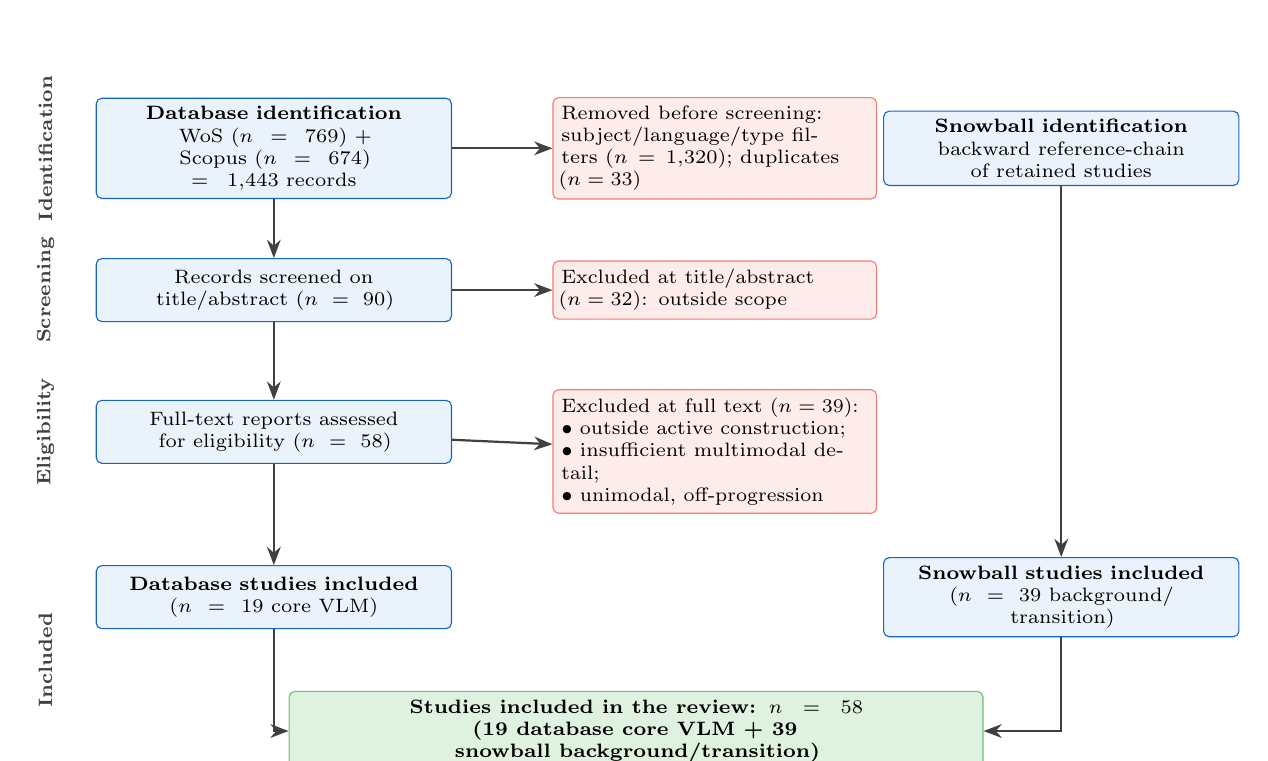
\begin{tikzpicture}[
  box/.style={rectangle, draw=prismabox, fill=lightblue!55, text width=4.3cm, align=center, minimum height=0.8cm, font=\scriptsize, rounded corners=2pt, inner sep=3pt},
  excl/.style={rectangle, draw=chartred!70, fill=chartred!10, text width=3.9cm, align=left, minimum height=0.7cm, font=\scriptsize, rounded corners=2pt, inner sep=3pt},
  final/.style={rectangle, draw=chartgreen!80, fill=chartgreen!18, text width=8.6cm, align=center, minimum height=0.9cm, font=\scriptsize\bfseries, rounded corners=2pt, inner sep=3pt},
  stage/.style={font=\scriptsize\bfseries\color{darkgray}, align=center, rotate=90},
  arr/.style={-Stealth, thick, color=darkgray},
]
% --- Database track (left) ---
\node[box] (dbid) at (0,0) {\textbf{Database identification}\\ WoS ($n=769$) + Scopus ($n=674$)\\ $=1{,}443$ records};
\node[excl] (dbpre) at (5.6,0) {Removed before screening: subject/language/type filters ($n=1{,}320$); duplicates ($n=33$)};
\node[box] (dbscr) at (0,-1.8) {Records screened on\\ title/abstract ($n=90$)};
\node[excl] (dbscrx) at (5.6,-1.8) {Excluded at title/abstract\\ ($n=32$): outside scope};
\node[box] (dbft) at (0,-3.6) {Full-text reports assessed\\ for eligibility ($n=58$)};
\node[excl] (dbftx) at (5.6,-3.85) {Excluded at full text ($n=39$):\\ $\bullet$ outside active construction;\\ $\bullet$ insufficient multimodal detail;\\ $\bullet$ unimodal, off-progression};
\node[box] (dbinc) at (0,-5.7) {\textbf{Database studies included}\\ ($n=19$ core VLM)};

% --- Snowball track (right) ---
\node[box] (sbid) at (10.0,0) {\textbf{Snowball identification}\\ backward reference-chain\\ of retained studies};
\node[box] (sbinc) at (10.0,-5.7) {\textbf{Snowball studies included}\\ ($n=39$ background/\\ transition)};

% --- Merge ---
\node[final] (final) at (4.6,-7.4) {Studies included in the review: $n=58$\\ (19 database core VLM + 39 snowball background/transition)};

% --- arrows ---
\draw[arr] (dbid) -- (dbpre);
\draw[arr] (dbid) -- (dbscr);
\draw[arr] (dbscr) -- (dbscrx);
\draw[arr] (dbscr) -- (dbft);
\draw[arr] (dbft) -- (dbftx);
\draw[arr] (dbft) -- (dbinc);
\draw[arr] (sbid) -- (sbinc);
\draw[arr] (dbinc.south) |- (final.west);
\draw[arr] (sbinc.south) |- (final.east);

% --- stage labels ---
\node[stage] at (-2.9,0) {Identification};
\node[stage] at (-2.9,-1.8) {Screening};
\node[stage] at (-2.9,-3.6) {Eligibility};
\node[stage] at (-2.9,-6.5) {Included};
\end{tikzpicture}
\end{figure}

\subsection{Data Charting and Extraction Process}

Following the selection of the 58 studies, a standardized data-extraction form was developed to chart the literature. As recommended by scoping-review methodology \cite{tricco2018}, the form was piloted on a subset of studies and iteratively refined to ensure that all variables addressing the research questions were captured consistently. The extracted data were organized into three analytical dimensions---Content Analysis, Technical Analysis, and Critical Analysis (Table~\ref{tab:charting}). Charting was performed by a single researcher (the author); no independent second reviewer or inter-rater reliability statistic (e.g., Cohen's $\kappa$) was computed, and the protocol was not pre-registered. This single-reviewer design introduces a risk of subjective classification bias---most acutely in paradigm assignment for architecturally borderline studies---which is acknowledged as a limitation (Section~\ref{sec:limitations}) and flagged as a priority for future work (Section~\ref{sec:nextsteps}). To mitigate it, paradigm assignments were cross-checked against the primary algorithm reported in each study, and the full charting record is reported transparently in the master table (Table~\ref{tab:master}) so that classifications are auditable.

\begin{table}[H]
\caption{Data Charting and Extraction Framework.}
\label{tab:charting}
\small
\rowcolors{2}{softgray}{white}
\begin{tabularx}{\textwidth}{L{2.6cm} L{4.5cm} Y}
\toprule
\rowcolor{lightblue}
\textbf{Analytical Dimension} & \textbf{Extraction Variables} & \textbf{Description}\\
\midrule
Content Analysis & Cluster/Application; Input Data; Spatiotemporal Task; Automation Level. & Identifies what the AI is doing by mapping the specific domain (e.g., safety vs.\ progress tracking), the sensory inputs utilized (e.g., video, image, point cloud), the specific spatiotemporal task (e.g., action recognition, tracking), and the system's level of autonomy (assistive vs.\ automated).\\
Technical Analysis & Algorithm/Model; Dataset; Validation Metric; Compute/Hardware. & Analyzes how the system operates by documenting the specific architectures (e.g., GPT-4o, CLIP), the nature of the training data (public vs.\ private/custom), the diverse evaluation metrics employed (e.g., mAP, F1-score), and the deployment environment (edge vs.\ cloud).\\
Critical Analysis & Key Limitation; Research Gap; Future Direction. & Evaluates the significance of the study by synthesizing the inherent technological or methodological bottlenecks, identifying unmet industry needs, and charting actionable future research trajectories.\\
\bottomrule
\end{tabularx}
\end{table}

\subsection{Data Synthesis}

Given the heterogeneous nature of the evaluation metrics across included studies---which range from geometric intersection-over-union (IoU) and mean average precision (mAP) measures \cite{nath2020,wang2024} to natural-language-generation metrics for image captioning such as BLEU, METEOR, and CIDEr \cite{jung2024,xiao2022}---a standardized quantitative meta-analysis was inappropriate. Instead, a thematic and narrative synthesis approach was adopted \cite{tricco2018}. The final corpus of 58 studies was thematically classified into three developmental stages: (1) the traditional baseline establishing the geometric--semantic disconnect, (2) the transitional bridge leveraging advanced but unimodal algorithms, and (3) the multimodal turn toward end-to-end Vision-Language Models (VLMs). This categorization forms the structural foundation for the descriptive and thematic analyses in Sections~3 and~4.

% ============================================================
\section{Descriptive Analysis of the Corpus}
% ============================================================

This section presents the descriptive mapping of the 58-study corpus, addressing the PRISMA-ScR requirement to characterize the volume, nature, and distribution of the included evidence. The analysis maps the literature across temporal, bibliometric, methodological, and topical dimensions, establishing the empirical foundation for the thematic analysis in Section~4. To keep the map focused on reader-relevant structure, descriptive dimensions that do not bear on the review's questions are reported compactly rather than exhaustively.

\subsection{Corpus Composition and Overview}

The final 58-study corpus is stratified into two methodological tiers: 39 background and transition studies (67.2\%) and 19 core construction VLM studies (32.8\%). The background/transition tier comprises 34 baseline studies---sensor-based tracking, unimodal computer vision, and NLP-based compliance systems---and 5 transitional ``bridging'' studies that deploy transformer-based architectures or hybrid CV--NLP pipelines preceding the full multimodal turn. The 19 core studies deploy CLIP, MLLM, captioning, and agentic hybrid stacks for active construction scene understanding.

\textbf{Analytical scope.} The full 58-study corpus is characterized descriptively to satisfy PRISMA-ScR's mapping requirement. The primary analytical sample for the thematic synthesis in Section~4, however, is the \textbf{19 core VLM studies} (supported by the 5 transition studies). The 34 backward-snowballed baseline studies establish the pre-VLM technological trajectory and serve as contextual reference rather than primary evidence. \textit{Taken together, the corpus is deliberately weighted: a small but rapidly growing core of genuine VLM applications, anchored by a substantial baseline that documents why the multimodal turn was necessary.}

\subsection{Publication Trends and Temporal Evolution}

Figure~\ref{fig:pubyear} plots the temporal distribution of the 58 studies on a continuous year axis, so the gaps between early baseline studies appear at their true scale. The earliest baseline anchors span 2009--2018 at one to four studies per year, reflecting the dominance of unimodal CV and sensor-based approaches. Output accelerates from 2021 (8 studies) and peaks in 2024 (12 studies), the year following the public release of large-scale multimodal foundation models (GPT-4V, CLIP, Florence-2, LLaVA), which sharply lowered the barrier to deploying VLMs on domain-specific tasks. The apparent decline in 2025 (6) and 2026 (2) is an artifact of the 4 March 2026 search cutoff---2025 indexing was still completing and 2026 captures barely two months---and should not be read as a genuine downturn. \textit{Taken together, the trend confirms that construction VLM research is a recent, foundation-model-driven phenomenon: more than two-thirds of the core studies appeared in 2024 or later, which both justifies a scoping (rather than systematic-comparative) review and signals that any map of this field is necessarily a snapshot of a fast-moving target.}

\begin{figure}[H]
\caption{Annual distribution of the 58 included studies (2009--2026), plotted on a continuous year axis. Years with no bar (e.g., 2010--2011, 2013--2014, 2016--2017) contained no included study. The 2025--2026 counts are truncated by the 4 March 2026 search cutoff.}
\label{fig:pubyear}
\centering
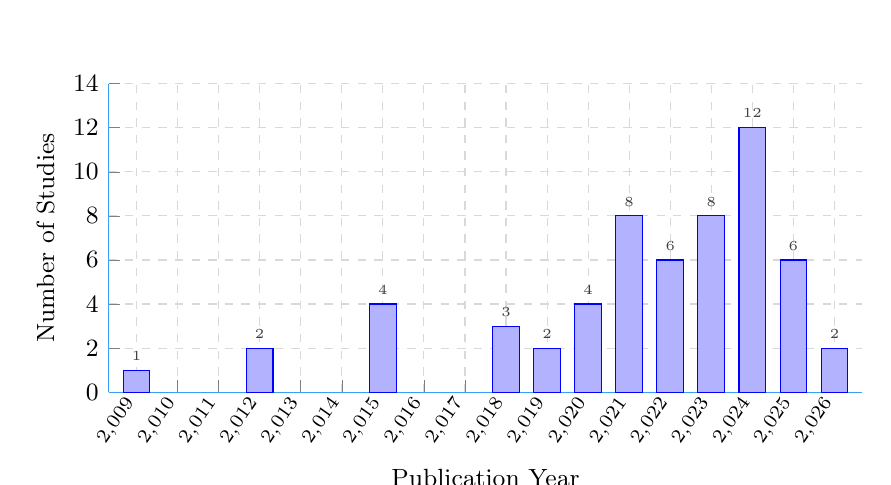
\begin{tikzpicture}
\begin{axis}[
  ybar,
  bar width=0.34cm,
  width=0.92\textwidth,
  height=5.5cm,
  xlabel={Publication Year},
  ylabel={Number of Studies},
  xtick={2009,2010,2011,2012,2013,2014,2015,2016,2017,2018,2019,2020,2021,2022,2023,2024,2025,2026},
  xticklabel style={rotate=55, anchor=east, font=\scriptsize},
  yticklabel style={font=\small},
  xlabel style={font=\small},
  ylabel style={font=\small},
  ymin=0, ymax=14,
  ytick={0,2,4,6,8,10,12,14},
  nodes near coords,
  nodes near coords style={font=\tiny, color=darkgray},
  axis lines*=left,
  enlarge x limits=0.04,
  fill=chartblue!70,
  draw=chartblue!90,
  tick align=inside,
  grid=major,
  grid style={dashed, gray!30},
]
\addplot coordinates {
  (2009,1) (2012,2) (2015,4) (2018,3) (2019,2) (2020,4) (2021,8) (2022,6) (2023,8) (2024,12) (2025,6) (2026,2)
};
\end{axis}
\end{tikzpicture}
\end{figure}

\subsection{Bibliometric Snapshot: Geography and Venues}

Two bibliometric dimensions---corresponding-author geography and publication venue---are reported compactly in Table~\ref{tab:biblio}, as neither bears directly on the review's architectural questions but both characterize the field's structure. Geographically, the corpus is concentrated in East Asia and North America: mainland China (17 studies, 29.3\%), the United States (14, 24.1\%), South Korea (9, 15.5\%), and Hong Kong (5, 8.6\%) together account for 77.6\% of the literature. By venue, the concentration is even sharper: \textit{Automation in Construction} alone published 36 of the 58 studies (62.1\%), with the remainder spread thinly across eleven other journals. \textit{Taken together, this dual concentration---geographic and editorial---means the field's evidence base is shaped by a small number of research groups publishing in a single dominant venue, a structural feature that the Discussion (Section~\ref{sec:discussion}) connects to the prevalence of private datasets and the absence of shared benchmarks.}

\begin{table}[H]
\caption{Bibliometric snapshot of the 58-study corpus: corresponding-author geography and top publication venues.}
\label{tab:biblio}
\small
\rowcolors{2}{softgray}{white}
\begin{tabularx}{\textwidth}{L{3.6cm} L{2.4cm} | L{4.6cm} L{2.4cm}}
\toprule
\rowcolor{lightblue}
\textbf{Country (primary author)} & \textbf{Studies (\%)} & \textbf{Publication venue} & \textbf{Studies (\%)}\\
\midrule
China (mainland) & 17 (29.3\%) & Automation in Construction & 36 (62.1\%)\\
United States & 14 (24.1\%) & J.\ Constr.\ Eng.\ Manage. & 5 (8.6\%)\\
South Korea & 9 (15.5\%) & Safety Science & 4 (6.9\%)\\
Hong Kong & 5 (8.6\%) & Computer-Aided Civ.\ Infr.\ Eng. & 3 (5.2\%)\\
Australia & 4 (6.9\%) & Advanced Eng.\ Informatics & 2 (3.4\%)\\
Canada & 2 (3.4\%) & J.\ Computing in Civil Eng. & 2 (3.4\%)\\
Other (7 countries) & 7 (12.1\%) & Other (6 journals) & 6 (10.3\%)\\
\bottomrule
\multicolumn{4}{l}{\small \textit{Totals:} $n=58$. Geography by primary corresponding-author institution; venue across 12 distinct journals.}
\end{tabularx}
\end{table}

\subsection{Study Characteristics: Application Domain and Automation Level}

Table~\ref{tab:appdomains} breaks down the 58 studies by application domain, automation level, and input modality. Safety applications account for 29 studies (50.0\%) and progress/activity tracking for 21 (36.2\%), with 5 (8.6\%) addressing both. The strong overall safety lean is driven by the baseline tier; within the 19 core VLM studies the balance inverts to progress-dominant (12 progress versus 7 safety), a divergence revisited in the thematic analysis. With respect to automation, the corpus is overwhelmingly automated (50 studies, 86.2\%); only 3 studies (5.2\%) deploy assistive, human-in-the-loop interfaces. By modality, images dominate (20, 34.5\%) but video and sequential frames are a substantial 18 studies (31.0\%), with image--text pairs at 10 (17.2\%).

\begin{table}[H]
\caption{Application domain, automation level, and input modality across the 58-study corpus.}
\label{tab:appdomains}
\small
\rowcolors{2}{softgray}{white}
\begin{tabularx}{\textwidth}{L{3.5cm} L{5.5cm} Y}
\toprule
\rowcolor{lightblue}
\textbf{Dimension} & \textbf{Category} & \textbf{Count (\%)}\\
\midrule
\rowcolor{lightblue!30}
\multicolumn{3}{l}{\small\bfseries Application Domain}\\
\rowcolor{white}
~ & Safety Management & 29 (50.0\%)\\
~ & Progress / Activity Tracking & 21 (36.2\%)\\
~ & Both (Combined) & 5 (8.6\%)\\
~ & Other (information/data mgmt, review) & 3 (5.2\%)\\
\midrule
\rowcolor{lightblue!30}
\multicolumn{3}{l}{\small\bfseries Automation Level}\\
\rowcolor{white}
~ & Fully Automated & 50 (86.2\%)\\
~ & Assistive (Human-in-Loop) & 3 (5.2\%)\\
~ & Other (manual / review / not applicable) & 5 (8.6\%)\\
\midrule
\rowcolor{lightblue!30}
\multicolumn{3}{l}{\small\bfseries Input Data Modality}\\
\rowcolor{white}
~ & Images Only & 20 (34.5\%)\\
~ & Video / Sequential Frames & 18 (31.0\%)\\
~ & Image + Text (VQA/Caption) & 10 (17.2\%)\\
~ & Images + Sensor / BIM / 3D & 5 (8.6\%)\\
~ & Other / mixed & 5 (8.6\%)\\
\bottomrule
\end{tabularx}
\end{table}

\textit{Taken together, two patterns stand out. First, the field's safety/progress balance is tier-dependent: baselines skew safety, but genuine VLM applications skew progress---so a title billing both domains equally is warranted only when the core is examined directly. Second, although video already constitutes nearly one-third of inputs, the corpus remains predominantly automated and image-centric, foreshadowing the underdeveloped temporal-reasoning capability identified in Section~\ref{sec:discussion}.}

\subsection{VLM Paradigm Distribution}

The 19 core VLM studies were classified according to the three-layered synthesis framework developed in Section~4.1. As shown in Table~\ref{tab:paradigms}, the three paradigms are near-evenly represented: Paradigm C (Hybrid Agentic systems fusing object detectors with MLLMs and ontologies) accounts for 7 studies (36.8\%), while Paradigm A (Zero/Few-Shot retrieval via CLIP, DINOv2, Florence-2) and Paradigm B (Domain Fine-Tuned generative captioning) account for 6 each (31.6\%). This balance reflects the field's simultaneous investment in three complementary capabilities---training-free flexibility, descriptive language generation, and interactive agentic reasoning---rather than convergence on a single approach. The 39 background and transition studies are classified separately as pre-VLM CV, sensor, or NLP systems. \textit{Taken together, the even paradigm split is the first quantitative signal that these architectures coexist rather than supersede one another---a point developed and visualized by publication year in Section~4.1.}

\begin{table}[H]
\caption{Distribution of the 19 core VLM studies across three architectural paradigms.}
\label{tab:paradigms}
\small
\rowcolors{2}{softgray}{white}
\begin{tabularx}{\textwidth}{L{4.2cm} L{2.2cm} Y L{3.5cm}}
\toprule
\rowcolor{lightblue}
\textbf{Paradigm} & \textbf{Studies ($n$)} & \textbf{Description} & \textbf{Representative Models}\\
\midrule
A: Zero/Few-Shot Retrieval & 6 (31.6\%) & Training-free; shared embedding space; cosine similarity matching. & CLIP, DINOv2, Florence-2, TIP-X\\
B: Domain Fine-Tuned Generative & 6 (31.6\%) & Supervised fine-tuning on construction datasets; encoder--decoder architectures. & CNN--LSTM, Transformer--SCST, VisualSiteDiary (mPLUG), Dense captioning\\
C: Hybrid Agentic / Geometric-Semantic & 7 (36.8\%) & MLLM + object detector fusion; ontology-guided prompting; interactive VQA. & YOLO + LLM, CogAgent + LoRA, Florence-2 + SAM2 + GPT-4o, Claude 3.7 + Robot\\
\midrule
Background / Transition & 39 & Unimodal CV, sensor-based, NLP-only, or transitional transformer systems. & YOLO, Faster R-CNN, BERT, knowledge graphs, TimeSformer, DART\\
\bottomrule
\multicolumn{4}{l}{\small Core VLM total: $n=19$ (A=6, B=6, C=7). Full corpus total: $n=58$.}
\end{tabularx}
\end{table}

\subsection{Evaluation Metrics Landscape}

A distinctive characteristic of this cross-disciplinary literature is the fragmentation of evaluation metrics. Table~\ref{tab:metrics} maps the evaluation approaches used across the 58 studies into four (non-exclusive) metric families. Detection and localization metrics (mAP, IoU, precision, recall, F1) are by far the most common, appearing in 35 studies where ground-truth bounding boxes are available. Classification metrics (accuracy, sensitivity, specificity) appear in 16 studies, spanning VQA binary checks and action recognition. Natural language generation (NLG) metrics (BLEU, CIDEr, SPICE, METEOR, ROUGE) appear in 6 studies, concentrated in the captioning-oriented Paradigm~B. User-study metrics (Likert scales, expert questionnaires) remain rare, appearing in only 2 studies despite their relevance to interactive agentic systems.

\begin{table}[H]
\caption{Evaluation Metric Families and Their Distribution Across the Corpus.}
\label{tab:metrics}
\small
\rowcolors{2}{softgray}{white}
\begin{tabularx}{\textwidth}{L{3.4cm} L{4.2cm} L{2.2cm} Y}
\toprule
\rowcolor{lightblue}
\textbf{Metric Family} & \textbf{Specific Metrics} & \textbf{Studies ($n$)} & \textbf{Typical Application Context}\\
\midrule
Detection / Localization & mAP, IoU, Precision, Recall, F1 & 35 & PPE detection, object recognition, activity classification\\
Classification & Accuracy, Sensitivity, Specificity, F1-score & 16 & VQA binary checks, compliance verification, action recognition\\
NLG / Captioning & BLEU, CIDEr, SPICE, METEOR, ROUGE & 6 & Image captioning, daily report generation, photolog retrieval\\
User Studies / Qualitative & Likert scale, expert questionnaire, BERTScore & 2 & Assistive systems, interactive chatbots, report usability\\
\bottomrule
\multicolumn{4}{l}{\small Note: metric families are non-exclusive; several studies report more than one, so counts do not sum to 58.}
\end{tabularx}
\end{table}

The absence of a shared benchmark is itself a finding. Across the 19 core VLM studies, 15 (79\%) evaluated on private or custom datasets unavailable for direct comparison; only 4 touched any public benchmark (e.g., SODA, ACID, TOCS), and even those do not share a common task specification or metric standard. \textit{Taken together, the metric landscape reveals a field that cannot yet measure its own progress: detection metrics dominate because they are inherited from the unimodal CV era, generation and human-centred metrics remain marginal despite the shift to language-producing systems, and the near-total reliance on private data makes cross-study comparison impossible.} This fragmentation, the most consequential descriptive finding of the review, is developed as a primary contribution in the Discussion (Section~\ref{sec:discussion}).

\subsection{Thematic Structure and Intellectual Bursts}

Beyond frequency counts, a scientometric analysis of author keywords and citation patterns exposes the intellectual structure underlying the corpus and provides an independent, citation-based check on the paradigm narrative. A keyword co-occurrence network of the 30 most frequent terms resolves, via modularity-based community detection, into four thematic clusters (Table~\ref{tab:thematic}). The most central terms by network betweenness are \textit{Hazard}, \textit{Object Detection}, \textit{Computer Vision}, and \textit{Image Captioning}---confirming that the field is organized around the tension between geometric perception (detection) and semantic description (captioning and hazard reasoning), the precise gap that the VLM paradigms address.

\begin{table}[H]
\caption{Thematic clusters from keyword co-occurrence analysis (modularity community detection over the 30 most frequent author keywords).}
\label{tab:thematic}
\small
\rowcolors{2}{softgray}{white}
\begin{tabularx}{\textwidth}{L{3.6cm} Y}
\toprule
\rowcolor{lightblue}
\textbf{Cluster (role)} & \textbf{Representative keywords}\\
\midrule
Detection core (motor theme) & Object Detection; Deep Learning; Few-Shot Learning; Machine Learning\\
Multimodal description (transversal) & Computer Vision; Image Captioning; Personal Protective Equipment; Zero-Shot Learning\\
Semantic reasoning (emerging) & Ontology; Hazard; Construction Safety; Identification\\
Sensing \& monitoring (niche) & Safety Monitoring; Infrastructure maintenance; IMU; 3D surveying\\
\bottomrule
\end{tabularx}
\end{table}

Citation-burst analysis---the temporary surges in how frequently a reference is cited---traces the field's shifting foundations. The strongest early bursts center on sensor- and detection-era anchors, including Costin (2012) on RFID resource tracking and Zhang (2015) on ontology-based compliance checking, whereas the most recent and still-active burst belongs to Wu (2021) on combining computer vision with semantic reasoning (active 2022--2024). \textit{Taken together, the scientometric structure corroborates the paradigm narrative from an independent vantage point: the intellectual base is migrating from a detection-and-ontology foundation toward integrated semantic reasoning---the very capability that defines the hybrid agentic systems of Paradigm~C.}

\subsection{Master Charting Table: All 24 Phase~1 Studies}

Table~\ref{tab:master} presents the complete data-charting results for all \textbf{24 Phase~1 studies}---19 core VLM studies and 5 transition/bridging studies. Each row maps a study to its paradigm, input modality, task, model architecture, dataset, validation metric, deployment environment, and key limitation, providing an auditable record of the primary analytical evidence base. The 34 backward-snowballed baseline studies are not charted here, as they serve only as contextual reference.

\begin{landscape}
\small
\rowcolors{2}{softgray}{white}
\begin{longtable}{L{2.8cm} L{1.7cm} L{2.0cm} L{2.5cm} L{1.5cm} L{3.0cm} L{1.8cm} L{2.0cm} L{2.0cm} L{3.2cm}}
\caption{Master data charting and technical synthesis of all 24 Phase~1 studies (19 core VLM + 5 transition). The arXiv preprint by Bui et al.\ (2026) is intentionally excluded (Section~2.2).}
\label{tab:master}\\
\toprule
\rowcolor{lightblue}
\textbf{Authors (Year)} & \textbf{Domain} & \textbf{Paradigm} & \textbf{Input Data} & \textbf{Task} & \textbf{Algorithm/Model} & \textbf{Dataset} & \textbf{Metric} & \textbf{Deployment} & \textbf{Key Limitation}\\
\midrule
\endfirsthead
\toprule
\rowcolor{lightblue}
\textbf{Authors (Year)} & \textbf{Domain} & \textbf{Paradigm} & \textbf{Input Data} & \textbf{Task} & \textbf{Algorithm/Model} & \textbf{Dataset} & \textbf{Metric} & \textbf{Deployment} & \textbf{Key Limitation}\\
\midrule
\endhead
\midrule
\endfoot
\bottomrule
\endlastfoot

% --- Paradigm A: Zero/Few-Shot ---
Zhang et al.\ (2025) & Progress & A (Zero-Shot) & Images & Object recognition & DINOv2, CLIP, TIP-X & SODA, ACID & mAP & Cloud/Edge & False positives from lack of domain-specific knowledge.\\

Gil \& Lee (2024) & Safety (PPE) & A (Zero-Shot) & Images & Zero-shot PPE monitoring & Image captioning + cosine sim. & Custom & Acc, F1, F2 & Cloud & Struggles with complex behaviors; limited domain vocab.\\

Liang et al.\ (2024) & Progress & A (Few-Shot) & Images & Few-shot object detection & CLIP + multimodal prototypes & SODA, TOCS & Accuracy & Cloud & Relies on similarity distributions; weak geometric precision.\\

Wang \& El-Gohary (2024) & Safety & A (Few-Shot) & Images & Few-shot detection + attribute recognition & Few-shot detector + attribute head & Custom site images & mAP, Precision, Recall & Cloud & Limited generalization to unseen construction classes.\\

Chen et al.\ (2023)~\cite{chenc2023} & Progress & A (Zero-Shot) & Video & Excavator productivity calculation & CLIP zero-shot + tracking & Custom & Accuracy (86\%), productivity (87.8\%) & Cloud & Activity recognition limited to one excavator type.\\

Sun et al.\ (2024)~\cite{sun2024} & Progress & A (Zero-Shot) & Images & Waste material recognition & VLM probing (GPT-4V, CLIP) & Custom waste dataset & Accuracy, F1 & Cloud & General VLMs underperform on fine-grained construction waste classes.\\

% --- Paradigm B: Domain Fine-Tuned ---
Liu et al.\ (2020) & Safety \& Progress & B (Fine-Tuned) & Images & Image captioning & CNN--LSTM & Dataset I \& II & BLEU, ROUGE, CIDEr & Cloud & Static descriptions; no interactive feedback capability.\\

Xiao et al.\ (2022) & Progress & B (Fine-Tuned) & Images & Object/action recognition \& captioning & Tsfm-SCST & ACID & Precision, Recall, F1 & Cloud & Lower F1 than traditional detectors for complex actions.\\

Zhai et al.\ (2023)~\cite{zhai2023} & Safety & B (Fine-Tuned) & Images & Unsafe behavior captioning & Transformer + attention & Custom & BLEU, Precision & Cloud & Limited sentence variation; annotation-quality dependent.\\

Wang Y. et al.\ (2024) & Safety & B (Fine-Tuned) & Image + Text & Visual-text semantic extraction & Transformer encoder + USE & ConDenseCap & Similarity matrix & Cloud & Challenges with sparse language in complex scenes.\\

Jung et al.\ (2024) & Progress (DCRs) & B (Fine-Tuned) & Photologs & Captioning \& retrieval & VisualSiteDiary (mPLUG) & VSD Dataset & BLEU, CIDEr, SPICE & Cloud & Grid features cause spatial information loss.\\

Bang \& Kim (2020)~\cite{bang2020} & Progress & B (Fine-Tuned) & UAV Images & Context-based captioning for UAV data & Dense captioning (CNN-based) & Custom UAV (1,431 images) & BLEU, METEOR & Cloud & Limited to static UAV frames; no temporal activity tracking.\\

% --- Paradigm C: Hybrid Agentic ---
Chen H. et al.\ (2024) & Safety & C (Hybrid) & Image + Text & VQA / retrieval (AR) & VLM + Augmented Reality & Custom & Recall@5, Accuracy & Edge (AR) & Reduced accuracy for complex ``danger type'' queries.\\

Hussain et al.\ (2026) & Safety & C (Hybrid) & Images & Hazard detection + dialogue & YOLO + LLM & Custom & BLEU, ROUGE, BERTScore & Mobile/Edge & Stability constrained by mobile device limits.\\

Chan et al.\ (2025) & Safety & C (Hybrid) & Image + Text & VQA / compliance & CogAgent + LoRA + Ontology & Custom & Sensitivity, F1 & Cloud & Continuous manual ontology updates required.\\

Xiao et al.\ (2024)~\cite{xiao2024} & Progress & C (Hybrid) & Video & Activity rec.\ + reporting & YOLO + 3D ResNet + ChatGPT & Custom & Likert (user exp.) & Cloud & Hallucinated outputs when historical data is sparse.\\

Jeoung et al.\ (2025) & Progress & C (Hybrid) & Video frames & Temporal event analysis & Florence-2 + SAM2 + GPT-4o & Custom MCQ & Accuracy, time & Cloud & Lower accuracy on complex temporal questions; prompt-sensitive.\\

Tuomisto et al.\ (2026) & Progress & C (Hybrid) & Images + BIM & Object presence detection & Claude 3.7 Sonnet + robot & Simulated \& real & Accuracy, Precision & Cloud/Edge & Dependent on high-LOD BIM accuracy; struggles with multi-stage elements.\\

Wang B. et al.\ (2024b)~\cite{wangb2024} & Progress & C (Hybrid) & Images + 3D & MEP scan-to-BIM & One-shot VFM + segmentation (Omni-Scan2BIM) & MEP scene dataset & Recognition acc. ($>$90\%) & Cloud & Limited to tubular MEP components; requires high-quality scans.\\

% --- Transition Papers ---
Yang et al.\ (2023)~\cite{yang2023} & Safety & Transition & Video & Unsafe behavior recognition & STR-Transformer & CMA Dataset & Loss, Accuracy & Cloud & High computational complexity limits real-time use.\\

Jang et al.\ (2025)~\cite{jang2025} & Progress & Transition & Video & Installation action recognition & VideoMAE V2, TimeSformer & PCI-Dataset & Accuracy (98.1\%), F1 & Cloud & Confusion between visually similar PC installation actions.\\

Xin et al.\ (2024)~\cite{xin2024} & Progress & Transition & Images & Automated object detection pipeline & DART (GroundingDINO + SDXL + InternVL) & Liebherr dataset & mAP, Precision & Cloud & Pipeline not construction-specific; requires domain prompt tuning.\\

Tohidifar et al.\ (2024)~\cite{tohidifar2024} & Safety \& Progress & Transition & Images (synth.) & Synthetic image + multimodal label generation & BlendCon framework (3D + GAN-style) & Synthetic (985,660 images) & AP@0.5--0.95 & Cloud & Synthetic-to-real domain gap; label fidelity varies with scene complexity.\\

Xiong et al.\ (2019) & Safety & Transition & Video & Hazard identification via visual relationships & Scene graph + relationship detection & Custom & Precision, Recall, F1 & Cloud & Semantic gap between visual relations and regulatory compliance rules.\\

\end{longtable}
\end{landscape}

% ============================================================
\section{Thematic Analysis: VLM Architectures and Construction Applications}
% ============================================================

Following the descriptive mapping in Section~3, this thematic analysis examines both the architectural mechanisms and the practical site applications of VLMs in active construction management. The following subsections map the cognitive-engine layer of the three-layered framework---directly addressing \textbf{RQ1} (prevalent VLM architectures) and \textbf{RQ2} (multimodal data fusion across safety and progress applications)---by tracing how visual and textual inputs are integrated across three architectural paradigms, synthesize the reported performance of those paradigms, and then examine how each paradigm's outputs translate into Layer~3 construction management deliverables, addressing \textbf{RQ3} (deployment barriers) and \textbf{RQ4} (evaluation) across the safety and progress domains.

\subsection{The Three-Layered Spatiotemporal VLM Framework}

For the purposes of this review, a Vision-Language Model (VLM) is defined as any architecture that jointly processes visual inputs (images, video frames, or point clouds) and natural language text within a shared representational space, enabling cross-modal tasks such as image captioning, visual question answering (VQA), and text-guided object detection. This definition encompasses contrastive alignment models (e.g., CLIP, DINOv2), generative encoder-decoder architectures (e.g., transformer-based captioning systems), and hybrid agentic stacks that pipeline object detectors with large language models. The terms ``multimodal large language model (MLLM)'' and ``Large Multimodal Model (LMM)'' are used interchangeably with VLM across the included literature; this review adopts VLM as the primary term.

To organize a heterogeneous and fast-moving literature, this review adopts a three-layered framework as a \emph{synthesis and classification tool} rather than as an original theoretical contribution. The framework borrows the familiar sensors--processors--actuators decomposition of automated decision-making \cite{parasuraman2000} and applies it to construction VLM systems; its value is not architectural novelty but the way it cleanly separates \emph{what enters} a system, \emph{how it reasons}, and \emph{what it delivers}, allowing studies built on very different models to be compared on common terms.

\textbf{Layer 1} is the sensory acquisition stage: raw visual streams, textual domain knowledge, and kinematic sensor data enter here. \textbf{Layer 2} is the VLM cognitive engine, where perception and semantic reasoning occur; because traditional scene graphs cannot capture the regulatory relationships needed for compliance checking \cite{wang2023}, this is precisely the layer the VLM paradigms transform. Layer~2 organizes the 19 core studies into three architectural paradigms: Zero/Few-Shot Prompting (Paradigm~A), Domain Fine-Tuned Generative Models (Paradigm~B), and Hybrid Geometric-Semantic Systems (Paradigm~C). \textbf{Layer 3} is the actuator stage, where Layer~2 outputs become construction management deliverables in the safety and progress domains.

Crucially, the A--B--C ordering is a \emph{typological} layering of capability---retrieval, then narration, then dialogue---not a strict chronological succession. As the paradigm-by-year distribution in Figure~\ref{fig:paradigmyear} shows, all three paradigms are active concurrently in the recent literature; each newer paradigm addresses a capability gap left by the previous one, but none has rendered the others obsolete. The framework emphasizes spatiotemporal analysis because construction job sites are highly dynamic, requiring models to track entities across both space and continuous time \cite{li2025}.

\begin{figure}[H]
\caption{Three-Layered Spatiotemporal VLM Framework for Construction Site Monitoring. Arrows show data flow from sensory inputs (Layer~1) through the cognitive engine (Layer~2) to construction management outputs (Layer~3).}
\label{fig:framework}
\centering
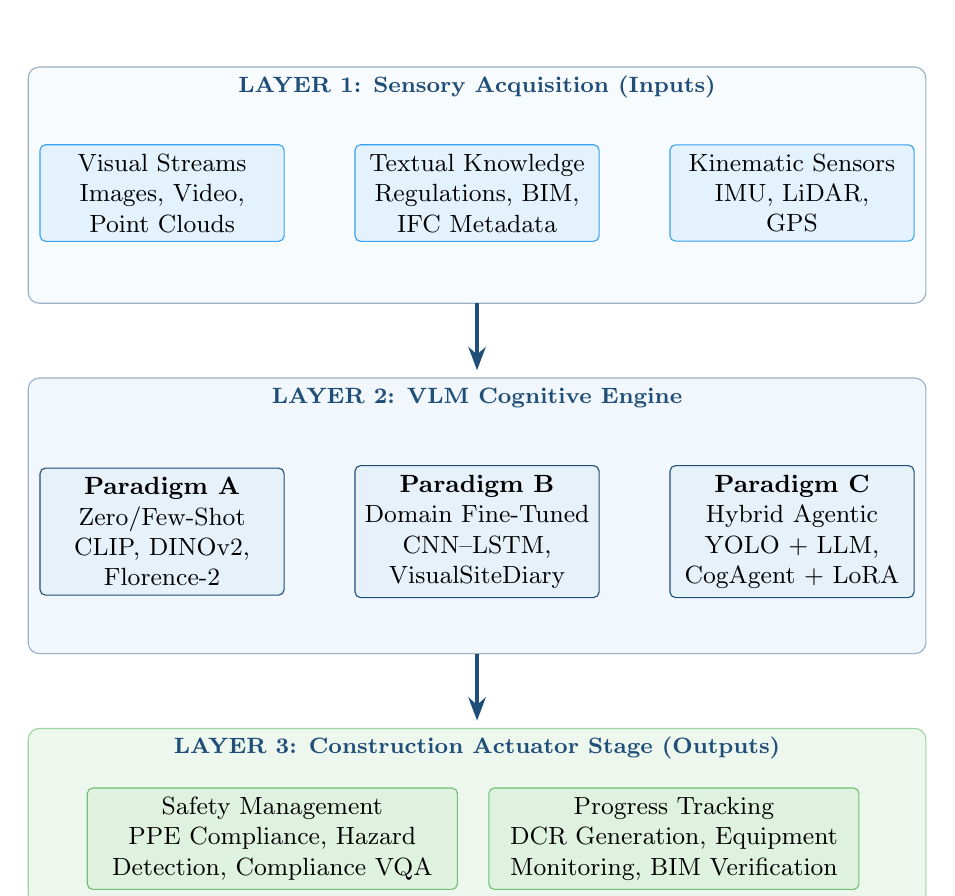
\begin{tikzpicture}[
  inp/.style={rectangle, draw=chartblue!90, fill=chartblue!12,
              rounded corners=2pt, minimum width=3.1cm, minimum height=1.1cm,
              align=center, font=\small},
  eng/.style={rectangle, draw=headingblue, fill=lightblue!65,
              rounded corners=2pt, minimum width=3.1cm, minimum height=1.6cm,
              align=center, font=\small},
  onode/.style={rectangle, draw=chartgreen!80, fill=chartgreen!18,
              rounded corners=2pt, minimum width=4.7cm, minimum height=1.2cm,
              align=center, font=\small},
  arr/.style={-Stealth, very thick, color=headingblue},
  hdr/.style={font=\footnotesize\bfseries\color{headingblue}},
]
%% --- Layer 1 background ---
\fill[lightblue!18, rounded corners=4pt] (-0.3, 1.0) rectangle (11.1, -2.0);
\draw[headingblue!45, rounded corners=4pt] (-0.3, 1.0) rectangle (11.1, -2.0);
\node[hdr] at (5.4, 0.75) {LAYER 1: Sensory Acquisition (Inputs)};

\node[inp] (i1) at (1.4, -0.6) {Visual Streams\\Images, Video,\\Point Clouds};
\node[inp] (i2) at (5.4, -0.6) {Textual Knowledge\\Regulations, BIM,\\IFC Metadata};
\node[inp] (i3) at (9.4, -0.6) {Kinematic Sensors\\IMU, LiDAR,\\GPS};

%% --- Arrow L1 → L2 ---
\draw[arr] (5.4,-2.0) -- (5.4,-2.85);

%% --- Layer 2 background ---
\fill[lightblue!38, rounded corners=4pt] (-0.3, -2.95) rectangle (11.1, -6.45);
\draw[headingblue!45, rounded corners=4pt] (-0.3, -2.95) rectangle (11.1, -6.45);
\node[hdr] at (5.4, -3.2) {LAYER 2: VLM Cognitive Engine};

\node[eng] (pa) at (1.4, -4.9) {\textbf{Paradigm A}\\Zero/Few-Shot\\CLIP, DINOv2,\\Florence-2};
\node[eng] (pb) at (5.4, -4.9) {\textbf{Paradigm B}\\Domain Fine-Tuned\\CNN--LSTM,\\VisualSiteDiary};
\node[eng] (pc) at (9.4, -4.9) {\textbf{Paradigm C}\\Hybrid Agentic\\YOLO + LLM,\\CogAgent + LoRA};

%% --- Arrow L2 → L3 ---
\draw[arr] (5.4,-6.45) -- (5.4,-7.3);

%% --- Layer 3 background ---
\fill[chartgreen!10, rounded corners=4pt] (-0.3, -7.4) rectangle (11.1, -9.65);
\draw[chartgreen!55, rounded corners=4pt] (-0.3, -7.4) rectangle (11.1, -9.65);
\node[hdr] at (5.4, -7.65) {LAYER 3: Construction Actuator Stage (Outputs)};

\node[onode] (o1) at (2.8, -8.8) {Safety Management\\PPE Compliance, Hazard\\Detection, Compliance VQA};
\node[onode] (o2) at (7.9, -8.8) {Progress Tracking\\DCR Generation, Equipment\\Monitoring, BIM Verification};
\end{tikzpicture}
\end{figure}

Figure~\ref{fig:paradigmyear} plots the 19 core studies by paradigm and publication year. The distribution makes the typological point concrete: domain fine-tuned captioning (Paradigm~B) appears earliest (from 2020), zero/few-shot retrieval (Paradigm~A) peaks in 2024, and hybrid agentic systems (Paradigm~C) emerge from 2024 and carry the most recent studies (2025--2026). Critically, 2024 contains all three paradigms simultaneously. \textit{Taken together, this confirms that the field is not replacing old paradigms with new ones but accumulating a layered repertoire---a researcher in 2025 may rationally choose a training-free retrieval model, a fine-tuned captioner, or an agentic stack depending on the task, which is why a chronological ``generations'' narrative would misrepresent the evidence.}

\begin{figure}[H]
\caption{Distribution of the 19 core VLM studies by architectural paradigm and publication year. All three paradigms are active concurrently (notably in 2024), supporting a typological rather than chronological interpretation.}
\label{fig:paradigmyear}
\centering
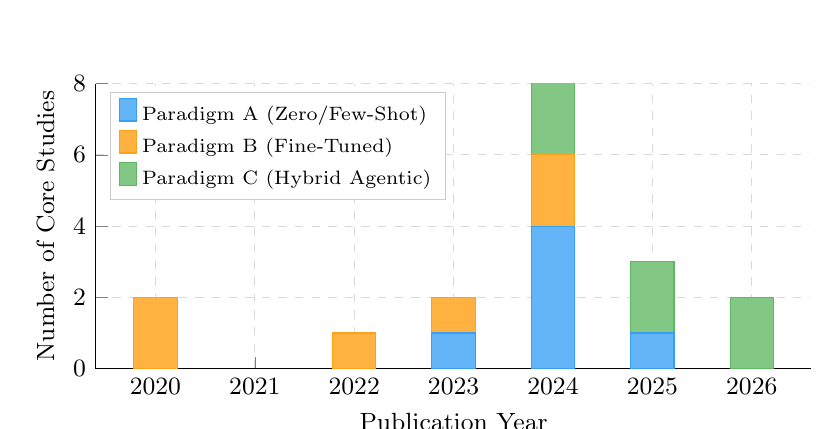
\begin{tikzpicture}
\begin{axis}[
  ybar stacked,
  bar width=0.55cm,
  width=0.88\textwidth,
  height=5.2cm,
  xlabel={Publication Year},
  ylabel={Number of Core Studies},
  symbolic x coords={2020,2021,2022,2023,2024,2025,2026},
  xtick=data,
  xticklabel style={font=\small},
  yticklabel style={font=\small},
  xlabel style={font=\small}, ylabel style={font=\small},
  ymin=0, ymax=8, ytick={0,2,4,6,8},
  legend style={at={(0.02,0.97)}, anchor=north west, font=\scriptsize, draw=gray!40},
  legend cell align=left,
  axis lines*=left, tick align=inside,
  grid=major, grid style={dashed, gray!30},
]
\addplot+[ybar, fill=chartblue!70, draw=chartblue!90] coordinates {(2020,0)(2021,0)(2022,0)(2023,1)(2024,4)(2025,1)(2026,0)};
\addplot+[ybar, fill=chartorange!75, draw=chartorange!90] coordinates {(2020,2)(2021,0)(2022,1)(2023,1)(2024,2)(2025,0)(2026,0)};
\addplot+[ybar, fill=chartgreen!70, draw=chartgreen!90] coordinates {(2020,0)(2021,0)(2022,0)(2023,0)(2024,3)(2025,2)(2026,2)};
\legend{Paradigm A (Zero/Few-Shot), Paradigm B (Fine-Tuned), Paradigm C (Hybrid Agentic)}
\end{axis}
\end{tikzpicture}
\end{figure}

\subsection{Paradigm A: Zero/Few-Shot Prompting (Retrieval-Oriented)}

The deployment of traditional computer vision on construction sites has historically been bottlenecked by the need for extensive annotated datasets. Because traditional supervised learning methods suffer from high annotation costs, severe computational demands, and limited datasets, scaling these systems to cover every potential hazard or piece of equipment has proven prohibitively labor-intensive \cite{zhang2025}. To circumvent this strict reliance on massive data collection, studies from 2022 onward increasingly deployed foundational VLMs, such as Contrastive Language-Image Pre-training (CLIP), DINOv2, and Florence-2. Rather than relying on rigid numerical labels defined during a lengthy training phase, these multimodal methods acquire generalized visual representations guided by natural language supervision, enabling impressive zero-shot detection capabilities without requiring task-specific retraining \cite{zhang2025}.

Zero-shot retrieval operates by embedding both visual and textual inputs into a shared semantic space, allowing natural language to guide visual perception without any domain-specific labeled data. Contrastive pre-training enables a model to recognize an unseen class from its text description alone \cite{gil2024}; cosine similarity between visual features and text prompts replaces the traditional classification head \cite{liang2024}. This architecture is task-agnostic by design: by altering the textual query, the same model can recognize temporary construction site objects \cite{liang2024}, track heavy earthmoving equipment states \cite{jeoung2025}, or verify PPE compliance through semantic similarity scoring \cite{gil2024}. Open-vocabulary models such as Florence-2 extend this further, detecting any object described in a natural language prompt without being constrained to predefined classes \cite{jeoung2025}.

Zero-shot retrieval solves data scarcity but introduces a new limitation: its output is always a label or a similarity score, never a sentence. Because these models output discrete object locations and isolated class tags, they cannot generate the human-readable narratives that site managers need to understand what is actually happening on site \cite{bui2026}. This descriptive ceiling (retrieval without narration) is the specific gap that Paradigm~B addresses through generative fine-tuning.

\subsection{Paradigm B: Domain Fine-Tuned Generative Models}

To overcome the descriptive gap left by zero-shot retrieval models, subsequent studies addressed this descriptive gap by adopting image captioning architectures. Unlike traditional object detection that merely outputs discrete labels, image captioning combines computer vision and NLP to translate visual information into comprehensive natural language descriptions \cite{liu2020}. Generative fine-tuning operates through an encoder-decoder framework: a visual encoder extracts image features and a language decoder generates natural language sequences \cite{xiao2022}. Training on domain-specific construction datasets allows these architectures to acquire construction vocabulary and translate complex site scenes into human-readable narratives \cite{liu2020}.

Generative language output unlocked two capabilities that zero-shot retrieval could not provide: proactive hazard documentation and automated daily reporting. For safety management, pairing object detection with captioning enabled systems to generate descriptive text that proactively identifies hazards by matching visual scene descriptions against text-based safety rules \cite{wangxiao2024}. For progress tracking, detector-free Vision-Language Transformer architectures such as VisualSiteDiary automatically caption site photologs, extracting actionable insights about the ``where,'' ``how,'' and ``what'' of daily construction activity to support Daily Construction Report generation \cite{jung2024}.

Generative fine-tuning produces richer output than retrieval, but it remains a one-way system: the model describes what it sees, and the user receives that description without recourse. Workers and inspectors need to ask follow-up questions and probe specific details---none of which a static captioning pipeline supports \cite{chen2024}. This interactivity gap (narration without dialogue) is what Paradigm~C resolves through agentic hybrid stacks.

\subsection{Paradigm C: Hybrid Geometric-Semantic Systems (Agentic \& Hybrid Stacks)}

To overcome the interactive bottleneck of static image captioning, recent studies deployed agentic Large Multimodal Models (MLLMs). While previous paradigms successfully described scenes, they struggled to correlate visual observations directly with complex regulatory codes due to inherent limitations in geometric reasoning \cite{hussain2026}. To bridge this gap, Paradigm C introduces hybrid frameworks that combine precise geometric reasoning (such as bounding box coordinates or Building Information Modeling data) with LLM-powered interpretation to achieve true, regulation-aware scene understanding \cite{hussain2026}.

Hybrid systems achieve regulation-aware reasoning by fusing geometric detection outputs with large language model interpretation. Object detectors---typically YOLO variants---extract precise bounding-box coordinates of workers and equipment, which are then formatted as structured text prompts and passed to an MLLM for semantic interpretation \cite{hussain2026}. This pipeline supports two-way interactive dialogue: the model generates safety captions and responds to follow-up queries in natural language \cite{hussain2026}. To prevent hallucination and enforce regulatory accuracy, researchers have embedded construction safety ontologies directly into the prompting framework, constraining the MLLM to industry-standard language and enabling multi-step compliance checks such as verifying three-point contact or secure anchorage attachment \cite{chan2025}.

Paradigm~C has extended VLM capability across both the temporal and spatial dimensions of site management. Temporally, processing multiple consecutive video frames enables spatial inference, task classification, and event-level analysis---allowing a model to determine not just what an excavator is, but what task it is performing and how long it has been idle \cite{jeoung2025}. Spatially, integrating a VLM with a quadruped robot and BIM data creates a fully autonomous inspection loop: as the robot navigates the site, the VLM compares captured images against IFC metadata to determine whether architectural elements are present and correctly installed \cite{tuomisto2026}.

However, while Paradigm C represents the most advanced tier of construction scene understanding, it carries notable vulnerabilities. The literature notes that despite progress in compliance checking, these models are still challenged by dynamic scenarios and complex behavioral detection \cite{hussain2026}. Their reliance on prompt engineering and their sensitivity to environmental noise also introduce new risks of latency and unreliability in safety-critical settings.

\subsection{Cross-Paradigm Performance Synthesis}

Having characterized the three paradigms qualitatively, this subsection synthesizes their reported quantitative performance (Table~\ref{tab:perf}). The exercise is revealing precisely because of what it cannot do. Where comparable accuracy-family numbers are reported, they cluster in a high band---Chen et al.\ (2023) report 86\% activity-recognition and 87.8\% productivity accuracy for zero-shot excavator monitoring; Chan et al.\ (2025) report 86.5\% sensitivity for ontology-guided work-at-height compliance; and Wang et al.\ (2024b) report over 90\% recognition accuracy for MEP scan-to-BIM. Among the transition studies, Jang et al.\ (2025) reach 98.1\% accuracy on precast-installation action recognition. Paradigm~B studies, by contrast, report natural-language-generation scores (BLEU, CIDEr, SPICE) that live on an entirely different scale.

The decisive observation is that \emph{these numbers cannot be pooled or ranked}. Each is measured on a different private dataset, against a different task definition, using a metric family appropriate to that task. An 86.5\% compliance sensitivity and a 98.1\% action-recognition accuracy are not on a common scale; a BLEU-4 captioning score and an mAP detection score are not even the same kind of quantity. \textit{Taken together, the inability to construct a defensible cross-study performance ranking is not a shortcoming of this synthesis but its central finding: the construction VLM field has demonstrated high headline accuracies in isolated settings, yet the absence of shared datasets and task definitions means no one---including a reviewer---can presently determine which paradigm performs best, or whether any system would hold up on another team's site.} This evaluation gap is developed as a primary contribution in Section~\ref{sec:discussion}.

\begin{table}[H]
\caption{Reported performance by paradigm, and why cross-study comparison is not defensible.}
\label{tab:perf}
\small
\rowcolors{2}{softgray}{white}
\begin{tabularx}{\textwidth}{L{2.6cm} L{3.0cm} L{4.4cm} Y}
\toprule
\rowcolor{lightblue}
\textbf{Paradigm} & \textbf{Dominant metrics} & \textbf{Selected reported results} & \textbf{Comparability}\\
\midrule
A: Zero/Few-Shot & mAP, accuracy, F1 & 86\% activity / 87.8\% productivity accuracy (Chen 2023); mAP gains on SODA/ACID (Zhang 2025, Liang 2024) & Different private/public datasets and tasks; not poolable\\
B: Fine-Tuned Generative & BLEU, CIDEr, SPICE, METEOR & Captioning scores on bespoke datasets (Liu 2020; Zhai 2023; Jung 2024) & NLG scores on incommensurable datasets; not poolable\\
C: Hybrid Agentic & Sensitivity, accuracy, Likert & 86.5\% compliance sensitivity (Chan 2025); $>$90\% MEP recognition (Wang 2024b); user studies (Xiao 2024) & Mixed objective/subjective metrics; not poolable\\
\midrule
\multicolumn{4}{l}{\small \textit{Finding:} no shared benchmark or task definition exists; reported accuracies cannot be ranked across studies.}\\
\bottomrule
\end{tabularx}
\end{table}

\subsection{Layer 3: Construction Site Applications}

The architectural paradigms mapped in Sections~4.2--4.4 define what a VLM can produce; the application domain determines what it should produce. Layer~3 of the Three-Layered Framework---the actuator stage---translates each paradigm's cognitive outputs into construction management deliverables. The architectural paradigm constrains what outputs are achievable. Zero-shot retrieval (Paradigm~A) supports object identification and compliance checks without labeled training data. Generative fine-tuning (Paradigm~B) enables descriptive site documentation and daily reporting. Hybrid agentic stacks (Paradigm~C) unlock interactive inspection, regulatory reasoning, and temporal event monitoring. The following two subsections examine how these outputs operate across the two principal site management domains covered by this review.

\subsubsection{Construction Safety and Risk Management}

PPE compliance was the first construction safety task to benefit from zero-shot retrieval, because it maps naturally onto text-visual matching: does the worker's appearance match a natural language description of required equipment? Paradigm~A systems achieved this without labeled training data by extracting skeletal key points, cropping body-part images, and comparing generated captions against OSHA regulation prompts via cosine similarity \cite{gil2024}. However, PPE presence alone does not establish safety: workers may be fully equipped yet still engage in high-risk behaviors arising from complex spatiotemporal interactions. Comprehensive hazard management therefore requires moving beyond object-level checks toward contextual behavioral analysis.

To comprehensively capture these risky interactions, subsequent studies deployed Paradigm~B domain fine-tuned generative models to analyze unsafe behaviors. By pairing object detection with image captioning, safety systems gained the ability to generate rich textual descriptions of active scenes. These descriptions were matched against text-based safety rules to proactively identify hazards \cite{wangxiao2024}. Yet, despite successfully generating descriptive safety narratives, these systems remained static and lacked context-specific, interactive feedback essential for workers to fully comprehend their surrounding environments \cite{chen2024}.

Where Paradigm~B systems produced static safety narratives, Paradigm~C hybrid systems enabled interactive, regulation-aware monitoring by combining geometric detection with conversational LLMs. Augmented Reality integration extended this further: the VCSQ system embeds real-time captioning and VQA into a head-mounted display, allowing workers to query surrounding hazards on demand rather than waiting for a centralized inspection cycle \cite{chen2024}. To prevent hallucination and enforce regulatory compliance, ontology-driven prompting frameworks inject construction safety knowledge directly into the model's context, enabling multi-step compliance verification such as work-at-height regulation checking \cite{chan2025}. Mobile deployment extended the same architecture to site inspectors, where object detection feeds geometric coordinates into an LLM to generate hazard captions and support interactive safety dialogue \cite{hussain2026}.

Despite this progression, current VLMs still struggle with nuanced behavioral interpretation. Distinguishing whether a crew is effectively collaborating or merely communicating in proximity remains beyond reliable automated assessment \cite{bui2026}. Safety and productivity, however, share the same visual scene. The architectural investments made for hazard detection---temporal reasoning, spatial grounding, language-guided querying---directly transfer to progress tracking, which the following subsection examines.

\subsubsection{Progress Tracking and Automated Reporting}

Automated progress tracking begins with a simpler problem than safety: locating resources on site. Zero-shot retrieval addresses this without annotation overhead by comparing visual features against open-source text labels. An ImageNet-based similarity cache combined with contrastive pre-training recognizes temporary construction objects with no task-specific retraining \cite{liang2024}. Training-free multimodal frameworks similarly fuse object detectors with foundation models to extract localized bounding boxes for specific tools and materials \cite{zhang2025}. However, knowing where a tool is does not explain what work is happening. This gap drove adoption of generative architectures for richer site understanding.

Automating the daily administrative burden of site logging required generative architectures capable of producing narrative-level descriptions rather than bounding boxes. Detector-free Vision-Language Transformers such as VisualSiteDiary fine-tune on diverse site photologs, extracting actionable insights about the ``where,'' ``how,'' and ``what'' of daily work to support automated Daily Construction Report generation \cite{jung2024}. The key advance of Paradigm~B for progress tracking is precisely this shift from detection to narration: the output---narratives, not bounding boxes---arrives ready for site managers to use without additional interpretation.

Daily snapshots, however, cannot capture construction progress as it actually unfolds over time. Long-horizon equipment monitoring requires processing sequential frames over minutes or hours, not isolated images. Zero-shot temporal frameworks address this by evaluating multiple-choice questions about spatial position, task state, and event timing. Without task-specific training, these models determine what an excavator is doing and when a dump truck sits idle \cite{jeoung2025}.

Temporal querying answers the what-and-when question for individual equipment units. Spatial completeness requires a different integration: confirming whether every architectural element across a floor plate is physically present and correctly installed demands site-level coverage that temporal analysis alone cannot provide. Recent automated inspection frameworks address this by coupling conversational MLLMs with quadruped robots and BIM data \cite{tuomisto2026}. As the robot navigates partially built environments, an integrated foundational vision-language model acts as a virtual inspector, analyzing visual data against metadata extracted directly from the Industry Foundation Classes (IFC) model. Comparing captured images against IFC metadata, the VLM delivers programmatic binary assessments on whether each element is present, correctly positioned, and properly installed. This process bridges the digital twin and physical reality in real time \cite{tuomisto2026}.

\textit{Taken together, progress tracking is where the construction VLM field is, in fact, most active: of the 19 core studies, 12 target progress and site-management tasks versus 7 targeting safety. The progress trajectory mirrors the safety trajectory exactly---retrieval for ``where'' (Paradigm~A), narration for ``what'' (Paradigm~B), and temporal/spatial reasoning for ``how and when'' (Paradigm~C)---which is why the same architectural investments serve both domains and why this review treats them as equal partners rather than treating progress as a secondary application of safety technology.}

% ============================================================
\section{Discussion and Limitations}
% ============================================================
\label{sec:discussion}

\subsection{Discussion}

Across 58 studies spanning 2009--2026, this review maps a layered repertoire of capabilities: from unimodal object detection and text-based compliance checking, through generative captioning and automated reporting, toward agentic hybrid systems capable of interactive, regulation-aware scene understanding. As Section~4.1 established, these capabilities accumulate rather than replace one another. The four research questions yield the following findings.

\textbf{RQ1 (Architectures):} The literature reveals three distinct architectural paradigms (Paradigm A--C), each representing a progressive resolution of the semantic gap between visual data and construction management meaning. Paradigm A (CLIP, DINOv2, Florence-2) resolved the data-scarcity problem through zero-shot and few-shot retrieval but remained limited to discrete object tags. Paradigm B (CNN--LSTM, transformer-based captioning) introduced generative language output, enabling human-readable scene descriptions and automated daily logs but lacked interactivity. Paradigm C (YOLO + MLLM + ontology hybrid stacks, BIM-integrated robot VLMs) represents the most architecturally complete tier, enabling multi-turn dialogue, compliance verification, and temporal event analysis. The field has thus moved from a single-modal localization paradigm toward a genuinely multimodal decision-support architecture. However, Paradigm C studies are still predominantly prototypes rather than deployed systems.

\textbf{RQ2 (Multimodal Data Fusion):} Across the 19 core VLM studies, structured visual--text fusion is the defining innovation, realized through three mechanisms: shared embedding spaces (Paradigm A), encoder--decoder text generation (Paradigm B), or detect-then-prompt pipelines (Paradigm C). At the corpus level, geometric and sensor modalities remain underrepresented: only 5 of 58 studies incorporate geometric sensor data (LiDAR, IMU, or BIM). Although video and sequential frames account for a substantial 18 of 58 studies, genuine \emph{temporal} reasoning over those frames is rare---most video studies still classify short clips rather than reason over long horizons. This shortfall directly shapes the field's weakness in long-horizon activity monitoring.

\textbf{RQ3 (Deployment Barriers):} Five recurring methodological bottlenecks emerge across the corpus. First, domain shift is the most universally reported limitation. This refers to the mismatch between models trained on general internet imagery and those deployed on construction sites, where object categories, lighting conditions, occlusion patterns, and domain terminology differ substantially. Second, data scarcity restricts the training and evaluation of domain-specific models; 15 of the 19 core VLM studies (79\%) relied on private custom datasets, preventing direct benchmarking. Third, prompt sensitivity in agentic Paradigm C systems introduces reliability risks in safety-critical contexts: minor prompt rewording can substantially alter model outputs. Fourth, real-site validation is systematically absent; the majority of studies evaluate on curated lab images or controlled video clips rather than unstructured field footage. Fifth, temporal reasoning remains the most technically underdeveloped capability. Understanding what is happening continuously over time, rather than at individual frames or short clips, is addressed by only one study in the corpus: Jeoung et al.\ (2025), which directly targets long-horizon equipment task monitoring.

\textbf{RQ4 (Evaluation):} Evaluation practice across the corpus is fragmented. No unified benchmark dataset or shared task specification exists for VLM-based construction monitoring. Detection metrics, NLG metrics, classification accuracy, and user studies are applied inconsistently across studies, making comparative assessment of progress impossible. The trend toward user-study evaluation in Paradigm C studies reflects a genuine shift toward human-centered assessment, but it introduces subjectivity and limits reproducibility. The absence of a shared benchmark reflects the field's immaturity. No agreed-upon task definitions yet exist for what ``good'' safety monitoring or progress tracking performance means in operational terms.

Taken together, these four findings point to a single overarching interpretation. The construction VLM field has demonstrated compelling proof-of-concept capability across safety inspection, progress reporting, PPE compliance, equipment monitoring, and interactive querying, but has not yet transitioned from laboratory demonstration to reliable field deployment. The practitioners' central question remains unanswered: can this system be trusted in an active construction environment? Human-in-the-loop deployment, with VLMs serving as assistive tools rather than autonomous decision-makers, is the most defensible near-term application model. This caution is reinforced by the one contextual data point outside the peer-reviewed corpus: an arXiv preprint probing whether general-purpose VLMs ``understand'' construction workers reports markedly low performance on domain-specific actions \cite{bui2026}, corroborating the domain-shift barrier---though, as a non-peer-reviewed source, it is treated as suggestive rather than confirmatory.

\subsection{Cross-Cutting Synthesis: Paradigm Meets Application}

Bridging the architectural analysis (Section~4) and the application analysis (Section~5) reveals patterns invisible to either alone. Table~\ref{tab:paradigmapp} cross-tabulates the 19 core studies by paradigm and primary application. Two findings stand out. First, \emph{every} paradigm is progress-leaning---Paradigms A and B each split 4 progress to 2 safety, and Paradigm C splits 4 to 3---so the field's safety reputation, inherited from the unimodal CV era, is not reflected in where VLM innovation is actually concentrated. Second, the most advanced capabilities are paradigm-locked: long-horizon temporal monitoring and BIM-integrated robotic inspection appear \emph{only} in Paradigm~C \cite{jeoung2025,tuomisto2026}, while no Paradigm~A or~B study attempts continuous temporal reasoning. \textit{Taken together, the architecture--application map shows that the field's frontier capabilities (temporal reasoning, autonomous inspection) are confined to its least mature, most prototype-heavy paradigm---which means the very capabilities practitioners most need for progress monitoring are precisely those with the least field validation.}

\begin{table}[H]
\caption{Cross-tabulation of the 19 core VLM studies by architectural paradigm and primary application.}
\label{tab:paradigmapp}
\small
\rowcolors{2}{softgray}{white}
\begin{tabularx}{\textwidth}{L{4.6cm} Y Y Y}
\toprule
\rowcolor{lightblue}
\textbf{Paradigm} & \textbf{Progress} & \textbf{Safety} & \textbf{Total}\\
\midrule
A: Zero/Few-Shot Retrieval & 4 & 2 & 6\\
B: Domain Fine-Tuned Generative & 4 & 2 & 6\\
C: Hybrid Agentic / Geometric-Semantic & 4 & 3 & 7\\
\midrule
\textbf{Total} & \textbf{12} & \textbf{7} & \textbf{19}\\
\bottomrule
\end{tabularx}
\end{table}

\subsection{Principal Contributions}

Against this synthesis, the review's two most consequential findings deserve to be named explicitly as contributions rather than left implicit in the analysis. \textbf{First, evaluation fragmentation is the field's binding constraint.} Because no shared benchmark or task definition exists and reported accuracies are measured on incommensurable private datasets (Section~4.5, Table~\ref{tab:perf}), the field cannot presently rank its own methods or substantiate progress claims---a structural problem more limiting than any single technical shortcoming. \textbf{Second, near-universal dataset privacy (79\% of core studies) compounds this constraint}, making results non-reproducible and tethering the literature to the small set of well-resourced groups identified in the bibliometric snapshot (Section~3.3). These two findings are mutually reinforcing: private data prevents shared benchmarks, and the absence of shared benchmarks removes the incentive to release data. Breaking this cycle is the single highest-leverage intervention available to the field, and it motivates the research agenda in Section~\ref{sec:nextsteps}.

\subsection{Limitations}
\label{sec:limitations}

Seven constraints should temper interpretation of these findings, each with a specific implication for how the results should be read.

\textit{Methodological scope.} As a scoping review, this study maps the extent and nature of the literature without appraising study quality, effect sizes, or the relative merit of specific architectures. Consequently, no claim is made about which paradigm ``works best''; the performance synthesis in Section~4.5 reports what studies claim, not which claims are most credible.

\textit{Database coverage.} Identification was restricted to Web of Science and Scopus. AI-venue papers indexed primarily in IEEE Xplore or the ACM Digital Library before WoS/Scopus coverage may be under-represented, which could disproportionately affect the most recent Paradigm~C systems that frequently debut in computer-science venues. Extending the search to these databases (Section~\ref{sec:nextsteps}) could add studies and shift the recency profile, though backward snowballing partially mitigates the gap.

\textit{Search recency.} The search was conducted on 4 March 2026. Given the field's publication pace---more than two-thirds of core studies appeared in 2024 or later---studies accepted after the cutoff are absent and some findings may already be superseded. The 2025--2026 counts in Figure~\ref{fig:pubyear} are correspondingly truncated and should not be read as a decline.

\textit{Geographic and linguistic concentration.} Mainland China ($n=17$), South Korea ($n=9$), and the United States ($n=14$) together account for 40 of 58 studies (69\%). Because building typologies, regulatory regimes (e.g., OSHA versus GB standards), and site practices differ across these settings, the mapped applications may not generalize globally. The English-language restriction compounds this: relevant Chinese- or Korean-language studies were excluded, and given that East Asian institutions dominate the corpus, the volume of missed non-English work may be substantial---a particularly important caveat for the safety-application mapping, where regulatory context is decisive.

\textit{Snowballing bias.} Backward snowballing, while necessary to recover foundational baselines, favors frequently cited earlier studies and may underrepresent newer, independently developed work that has not yet accumulated citations---potentially understating the diversity of very recent approaches.

\textit{Absence of quality appraisal.} Consistent with scoping-review method, all included studies are treated as evidentiarily equivalent regardless of sample size, validation rigor, or peer-review status. This is a genuine limitation: a small probing study and an extensively validated system paper carry equal weight in the descriptive map. Readers should not infer that equal treatment implies equal evidential strength, and a future systematic review with formal quality appraisal would be needed before any ``which approach works'' conclusion.

\textit{Single-reviewer charting.} Screening and data charting were performed by one researcher without an independent second reviewer or an inter-rater reliability statistic, introducing a risk of subjective classification bias---most acutely in assigning architecturally borderline studies to paradigms. Paradigm assignments were cross-checked against each study's primary reported algorithm and the full charting is auditable in Table~\ref{tab:master}, but dual-reviewer charting (Section~\ref{sec:nextsteps}) would strengthen reliability.

% ============================================================
\section{Next Steps}
\label{sec:nextsteps}
% ============================================================

This review represents the current, strongest stage of an ongoing project rather than a finished systematic review, and several concrete steps would extend and strengthen it.

\textbf{Completing the review methodology.} Three methodological extensions are planned. First, the identification stage will be broadened beyond Web of Science and Scopus to \textbf{IEEE Xplore}, and potentially the ACM Digital Library and the ASCE Library, using the identical Boolean strings; the additional records will be reconciled into an updated PRISMA flow and the descriptive distributions recomputed. This directly addresses the database-coverage limitation and is expected most to affect the recent Paradigm~C studies. Second, a \textbf{second independent reviewer} will re-screen and re-chart a sample of the corpus so that an inter-rater reliability statistic (Cohen's $\kappa$) can be reported and paradigm assignments for borderline studies verified. Third, \textbf{forward snowballing} (citing-article tracking) will complement the backward snowballing used here, reducing the bias toward established references and capturing the newest independent work.

\textbf{Maintaining currency.} Because the field is moving quickly and the corpus is a snapshot as of March 2026, the search will be re-run periodically, and the arXiv preprints retained only as contextual evidence (e.g., Bui et al.) will be tracked to their peer-reviewed versions and promoted into the counted corpus once published.

\textbf{Strengthening the field (agenda for the community).} The review's findings define a near-term research agenda whose highest-leverage item is unambiguous: a \textbf{shared, public, construction-specific VLM benchmark}. Such a benchmark should span safety compliance, equipment task classification, and long-horizon temporal activity chains, be drawn from real (not laboratory) sites, and standardize task definitions and metrics so that the cross-study comparison shown to be impossible in Section~4.5 becomes feasible. Alongside it, the field needs (i) a deliberate investment in \textbf{temporal reasoning} over video, currently confined to a single core study; (ii) \textbf{real-site validation protocols} that move evaluation off curated clips and onto unstructured field footage; and (iii) \textbf{standardized reporting} of datasets, prompts, and metrics to make agentic results reproducible. Progress on the benchmark would, by itself, unlock most of the others.

% ============================================================
\section{Conclusion}
% ============================================================

This scoping review mapped 58 peer-reviewed studies to characterize the current state of Vision-Language Model (VLM) and multimodal AI applications for construction site safety monitoring and progress tracking. The review reveals a field accumulating a layered repertoire of multimodal capabilities that fuse visual perception with natural language reasoning, organized here into three architectural paradigms that coexist rather than supersede one another: retrieval-oriented zero-shot models that use language to guide visual search; generative domain-fine-tuned captioning pipelines that produce human-readable site reports; and agentic hybrid stacks that integrate object detectors, large multimodal models, and domain ontologies into interactive, regulation-aware inspection systems.

The review makes three contributions. First, as positioned against eight prior reviews in Table~\ref{tab:priorreviews}, it is---to the authors' knowledge---the first PRISMA-ScR scoping review to map VLM architectural-paradigm evolution across \emph{both} construction safety and progress monitoring, organized through a three-layered framework (sensory inputs, cognitive engine, actionable outputs) offered as a reusable synthesis and classification tool rather than a novel theory. Second, it answers four research questions covering architectural prevalence, multimodal fusion, deployment barriers, and evaluation practice, and it adds a quantitative cross-paradigm synthesis (Section~4.5) and a paradigm-by-application cross-tabulation (Section~\ref{sec:discussion}) that prior reviews do not provide. Third, and most consequentially, it names two structural findings as the field's binding constraints: \emph{evaluation fragmentation}---no shared benchmark exists and reported accuracies cannot be ranked across studies---and \emph{near-universal dataset privacy} (79\% of core studies), which together prevent the field from substantiating its own progress claims. Alongside these, the review documents the underdevelopment of long-horizon temporal reasoning and the systematic absence of real-site validation.

These findings carry a clear practical message. The most actionable items are detailed as a research agenda in Section~\ref{sec:nextsteps}, foremost among them a shared, public, construction-specific benchmark. For practitioners, the current evidence base supports VLMs as assistive inspection tools with mandatory human verification for safety-critical decisions; full-autonomy deployment remains premature given prevailing prompt sensitivity, domain shift, and the scarcity of real-site reliability data. In sum, VLMs represent substantial progress over their unimodal predecessors, yet a clear distance remains before the technology delivers reliable, field-validated performance across the diversity of real construction environments.

\begin{thebibliography}{99}

\bibitem{alaloul2022} Alaloul, W.~S., Alzubi, K.~M., Malkawi, A.~B., Al Salaheen, M., and Musarat, M.~A. (2022). ``Productivity monitoring in building construction projects: A systematic review.'' \textit{Engineering, Construction and Architectural Management}, 29(7), 2760--2785. \href{https://doi.org/10.1108/ECAM-03-2021-0211}{DOI: 10.1108/ECAM-03-2021-0211}

\bibitem{asadzadeh2020} Asadzadeh, A., Arashpour, M., Li, H., Ngo, T., Bab-Hadiashar, A., and Rashidi, A. (2020). ``Sensor-based safety management.'' \textit{Automation in Construction}, 113, 103128. \href{https://doi.org/10.1016/j.autcon.2020.103128}{DOI: 10.1016/j.autcon.2020.103128}

\bibitem{bang2020} Bang, S., and Kim, H. (2020). ``Context-based information generation for managing UAV-acquired data using image captioning.'' \textit{Automation in Construction}, 112, 103116. \href{https://doi.org/10.1016/j.autcon.2020.103116}{DOI: 10.1016/j.autcon.2020.103116}

\bibitem{bohn2010} Bohn, J.~S., and Teizer, J. (2010). ``Benefits and barriers of construction project monitoring using high-resolution automated cameras.'' \textit{Journal of Construction Engineering and Management}, 136(6), 632--640. \href{https://doi.org/10.1061/(ASCE)CO.1943-7862.0000167}{DOI: 10.1061/(ASCE)CO.1943-7862.0000167}

\bibitem{bui2026} Bui, H.~T., Chodosh, N.~E., and Tavakoli, A. (2026). ``Can vision-language models understand construction workers? An exploratory study.'' arXiv preprint arXiv:2601.10835. \href{https://arxiv.org/abs/2601.10835}{arXiv: 2601.10835}

\bibitem{chan2025} Chan, C.-F., Wong, P.~K.-Y., Guo, X., Cheng, J.~C.~P., Chan, J.~P.-C., Leung, P.-H., and Tao, X. (2025). ``Context-aware vision-language model agent enriched with domain-specific ontology for construction site safety monitoring.'' \textit{Automation in Construction}, 177, 106305. \href{https://doi.org/10.1016/j.autcon.2025.106305}{DOI: 10.1016/j.autcon.2025.106305}

\bibitem{chenc2023} Chen, C., Xiao, B., Zhang, Y., and Zhu, Z. (2023). ``Automatic vision-based calculation of excavator earthmoving productivity using zero-shot learning activity recognition.'' \textit{Automation in Construction}, 146, 104702. \href{https://doi.org/10.1016/j.autcon.2022.104702}{DOI: 10.1016/j.autcon.2022.104702}

\bibitem{chen2024} Chen, H., Hou, L., Wu, S., Zhang, G., Zou, Y., Moon, S., and Bhuiyan, M. (2024). ``Augmented reality, deep learning and vision-language query system for construction worker safety.'' \textit{Automation in Construction}, 157, 105158. \href{https://doi.org/10.1016/j.autcon.2023.105158}{DOI: 10.1016/j.autcon.2023.105158}

\bibitem{davila2021} Davila Delgado, J.~M., and Oyedele, L. (2021). ``Deep learning with small datasets: Using autoencoders to address limited datasets in construction management.'' \textit{Applied Soft Computing}, 112, 107836. \href{https://doi.org/10.1016/j.asoc.2021.107836}{DOI: 10.1016/j.asoc.2021.107836}

\bibitem{gil2024} Gil, M., and Lee, S. (2024). ``Zero-shot monitoring of construction workers' personal protective equipment based on image captioning.'' \textit{Automation in Construction}, 164, 105470. \href{https://doi.org/10.1016/j.autcon.2024.105470}{DOI: 10.1016/j.autcon.2024.105470}

\bibitem{hussain2026} Hussain, R., Lee, D., Abbas, M.~S., Zaidi, S.~F.~A., Pedro, A., and Park, C. (2026). ``Vision-language model-based intelligent assistant for onsite construction safety inspection.'' \textit{Automation in Construction}, 182, 106728. \href{https://doi.org/10.1016/j.autcon.2025.106728}{DOI: 10.1016/j.autcon.2025.106728}

\bibitem{jang2025} Jang, J., Cha, M., Park, M., and Kim, H. (2025). ``Transformer-based deep learning model and video dataset for installation action recognition in offsite projects.'' \textit{Automation in Construction}, 172, 106042. \href{https://doi.org/10.1016/j.autcon.2025.106042}{DOI: 10.1016/j.autcon.2025.106042}

\bibitem{jeoung2025} Jeoung, H., Jung, M., and Kim, C. (2025). ``Zero-shot framework for construction equipment task monitoring.'' \textit{Computer-Aided Civil and Infrastructure Engineering}. \href{https://doi.org/10.1111/mice.13506}{DOI: 10.1111/mice.13506}

\bibitem{jiang2023} Jiang, Z., and Messner, J.~I. (2023). ``Computer vision applications in construction and asset management phases: A literature review.'' \textit{Journal of Information Technology in Construction (ITcon)}, 28(9), 176--199. \href{https://doi.org/10.36680/j.itcon.2023.009}{DOI: 10.36680/j.itcon.2023.009}

\bibitem{jung2024} Jung, Y., Cho, I., Hsu, S.-H., and Golparvar-Fard, M. (2024). ``VisualSiteDiary: A detector-free vision-language transformer model for captioning photologs for daily construction reporting and image retrievals.'' \textit{Automation in Construction}, 165, 105483. \href{https://doi.org/10.1016/j.autcon.2024.105483}{DOI: 10.1016/j.autcon.2024.105483}

\bibitem{li2025} Li, H., Deng, H., and Deng, Y. (2025). ``Towards worker-centric construction scene understanding: Status quo and future directions.'' \textit{Automation in Construction}, 171, 106005. \href{https://doi.org/10.1016/j.autcon.2025.106005}{DOI: 10.1016/j.autcon.2025.106005}

\bibitem{liang2024} Liang, Y., et al. (2024). ``Recognizing temporary construction site objects using CLIP-based few-shot learning and multi-modal prototypes.'' \textit{Automation in Construction}, 165, 105542. \href{https://doi.org/10.1016/j.autcon.2024.105542}{DOI: 10.1016/j.autcon.2024.105542}

\bibitem{liu2020} Liu, H., Wang, G., Huang, T., He, P., Skitmore, M., and Luo, X. (2020). ``Manifesting construction activity scenes via image captioning.'' \textit{Automation in Construction}, 119, 103334. \href{https://doi.org/10.1016/j.autcon.2020.103334}{DOI: 10.1016/j.autcon.2020.103334}

\bibitem{nath2020} Nath, N.~D., Behzadan, A.~H., and Paal, S.~G. (2020). ``Deep learning for site safety: Real-time detection of personal protective equipment.'' \textit{Automation in Construction}, 112, 103085. \href{https://doi.org/10.1016/j.autcon.2020.103085}{DOI: 10.1016/j.autcon.2020.103085}

\bibitem{paneru2021} Paneru, S., and Jeelani, I. (2021). ``Computer vision applications in construction: Current state, opportunities \& challenges.'' \textit{Automation in Construction}, 132, 103940. \href{https://doi.org/10.1016/j.autcon.2021.103940}{DOI: 10.1016/j.autcon.2021.103940}

\bibitem{parasuraman2000} Parasuraman, R., Sheridan, T.~B., and Wickens, C.~D. (2000). ``A model for types and levels of human interaction with automation.'' \textit{IEEE Transactions on Systems, Man, and Cybernetics -- Part A}, 30(3), 286--297. \href{https://doi.org/10.1109/3468.844354}{DOI: 10.1109/3468.844354}

\bibitem{rabbi2024} Rabbi, A.~B.~K., and Jeelani, I. (2024). ``AI integration in construction safety: Current state, challenges, and future opportunities in text, vision, and audio based applications.'' \textit{Automation in Construction}, 164, 105443. \href{https://doi.org/10.1016/j.autcon.2024.105443}{DOI: 10.1016/j.autcon.2024.105443}

\bibitem{samsami2024} Samsami, R. (2024). ``A systematic review of automated construction inspection and progress monitoring (ACIPM): Applications, challenges, and future directions.'' \textit{CivilEng}, 5(1), 265--287. \href{https://doi.org/10.3390/civileng5010014}{DOI: 10.3390/civileng5010014}

\bibitem{sherafat2020} Sherafat, B., Ahn, C.~R., Akhavian, R., Behzadan, A.~H., Golparvar-Fard, M., Kim, H., Lee, Y.-C., Rashidi, A., and Rezazadeh Azar, E. (2020). ``Automated methods for activity recognition of construction workers and equipment: State-of-the-art review.'' \textit{Journal of Construction Engineering and Management}, 146(6), 03120002. \href{https://doi.org/10.1061/(ASCE)CO.1943-7862.0001843}{DOI: 10.1061/(ASCE)CO.1943-7862.0001843}

\bibitem{sun2024} Sun, Y., Gu, Z., and Yang, S.~B. (2024). ``Probing vision and language models for construction waste material recognition.'' \textit{Automation in Construction}, 166, 105629. \href{https://doi.org/10.1016/j.autcon.2024.105629}{DOI: 10.1016/j.autcon.2024.105629}

\bibitem{tohidifar2024} Tohidifar, A., Kim, D., and Lee, S. (2024). ``Make it till you fake it: Construction-centric computational framework for simultaneous image synthetization and multimodal labeling.'' \textit{Automation in Construction}, 167, 105696. \href{https://doi.org/10.1016/j.autcon.2024.105696}{DOI: 10.1016/j.autcon.2024.105696}

\bibitem{tricco2018} Tricco, A.~C., Lillie, E., Zarin, W., O'Brien, K.~K., et al. (2018). ``PRISMA extension for scoping reviews (PRISMA-ScR): Checklist and explanation.'' \textit{Annals of Internal Medicine}, 169(7), 467--473. \href{https://doi.org/10.7326/M18-0850}{DOI: 10.7326/M18-0850}

\bibitem{tuomisto2026} Tuomisto, J., Zheng, Y., Chauhan, I., Sepp\"anen, O., and Pajarinen, J. (2026). ``Automating on-site object inspection with a quadruped robot and BIM.'' \textit{Automation in Construction}, 181, 106571. \href{https://doi.org/10.1016/j.autcon.2025.106571}{DOI: 10.1016/j.autcon.2025.106571}

\bibitem{wang2023} Wang, X., and El-Gohary, N. (2023). ``Deep learning-based relation extraction and knowledge graph-based representation of construction safety requirements.'' \textit{Automation in Construction}, 147, 104696. \href{https://doi.org/10.1016/j.autcon.2022.104696}{DOI: 10.1016/j.autcon.2022.104696}

\bibitem{wang2024} Wang, X., and El-Gohary, N. (2024). ``Few-shot object detection and attribute recognition from construction site images for improved field compliance.'' \textit{Automation in Construction}, 167, 105539. \href{https://doi.org/10.1016/j.autcon.2024.105539}{DOI: 10.1016/j.autcon.2024.105539}

\bibitem{wangb2024} Wang, B., Chen, Z., Li, M., Wang, Q., Yin, C., and Cheng, J.~C.~P. (2024). ``Omni-Scan2BIM: A ready-to-use Scan2BIM approach based on vision foundation models for MEP scenes.'' \textit{Automation in Construction}, 162, 105384. \href{https://doi.org/10.1016/j.autcon.2024.105384}{DOI: 10.1016/j.autcon.2024.105384}

\bibitem{wangxiao2024} Wang, Y., Xiao, B., Bouferguene, A., and Al-Hussein, M. (2024). ``Proactive safety hazard identification using visual--text semantic similarity for construction safety management.'' \textit{Automation in Construction}, 166, 105602. \href{https://doi.org/10.1016/j.autcon.2024.105602}{DOI: 10.1016/j.autcon.2024.105602}

\bibitem{wu2021} Wu, H., Zhong, B., Li, H., Love, P., Pan, X., and Zhao, N. (2021). ``Combining computer vision with semantic reasoning for on-site safety management in construction.'' \textit{Journal of Building Engineering}, 42, 103036. \href{https://doi.org/10.1016/j.jobe.2021.103036}{DOI: 10.1016/j.jobe.2021.103036}

\bibitem{xiao2022} Xiao, B., Wang, Y., and Kang, S.-C. (2022). ``Deep learning image captioning in construction management: A feasibility study.'' \textit{Journal of Construction Engineering and Management}, 148(7), 04022049. \href{https://doi.org/10.1061/(ASCE)CO.1943-7862.0002297}{DOI: 10.1061/(ASCE)CO.1943-7862.0002297}

\bibitem{xiao2024} Xiao, B., Wang, Y., Zhang, Y., Chen, C., and Darko, A. (2024). ``Automated daily report generation from construction videos using ChatGPT and computer vision.'' \textit{Automation in Construction}, 168, 105874. \href{https://doi.org/10.1016/j.autcon.2024.105874}{DOI: 10.1016/j.autcon.2024.105874}

\bibitem{xin2024} Xin, C., Hartel, A., and Kasneci, E. (2024). ``DART: An automated end-to-end object detection pipeline with data diversification, open-vocabulary bounding box annotation, pseudo-label review, and model training.'' \textit{Expert Systems with Applications}, 258, 125124. \href{https://doi.org/10.1016/j.eswa.2024.125124}{DOI: 10.1016/j.eswa.2024.125124}

\bibitem{xiong2019} Xiong, R., Song, Y., Li, H., and Wang, Y. (2019). ``Onsite video mining for construction hazards identification with visual relationships.'' \textit{Advanced Engineering Informatics}, 42, 100966. \href{https://doi.org/10.1016/j.aei.2019.100966}{DOI: 10.1016/j.aei.2019.100966}

\bibitem{yang2023} Yang, M., Wu, C., Guo, Y., Jiang, R., Zhou, F., Zhang, J., and Yang, Z. (2023). ``Transformer-based deep learning model and video dataset for unsafe action identification in construction projects.'' \textit{Automation in Construction}, 146, 104703. \href{https://doi.org/10.1016/j.autcon.2022.104703}{DOI: 10.1016/j.autcon.2022.104703}

\bibitem{zhai2023} Zhai, P., Wang, J., and Zhang, L. (2023). ``Extracting worker unsafe behaviors from construction images using image captioning with deep learning--based attention mechanism.'' \textit{Journal of Construction Engineering and Management}, 149(2), 04022164. \href{https://doi.org/10.1061/JCEMD4.COENG-12096}{DOI: 10.1061/JCEMD4.COENG-12096}

\bibitem{zhang2015} Zhang, J., and El-Gohary, N.~M. (2015). ``Automated information transformation for automated regulatory compliance checking in construction.'' \textit{Journal of Computing in Civil Engineering}, 29(4), B4015001. \href{https://doi.org/10.1061/(ASCE)CP.1943-5487.0000427}{DOI: 10.1061/(ASCE)CP.1943-5487.0000427}

\bibitem{zhang2025} Zhang, Z., Yu, Y., Pan, Z., and Antwi-Afari, M.~F. (2025). ``Training-free few-shot construction tool and material detection using pre-trained vision-language model.'' \textit{Computer-Aided Civil and Infrastructure Engineering}, 40(30), 6004--6023. \href{https://doi.org/10.1111/mice.13326}{DOI: 10.1111/mice.13326}

\bibitem{zhong2019} Zhong, B., Wu, H., Ding, L., Love, P.~E.~D., Li, H., Luo, H., and Jiao, L. (2019). ``Mapping computer vision research in construction: Developments, knowledge gaps and implications for research.'' \textit{Automation in Construction}, 107, 102919. \href{https://doi.org/10.1016/j.autcon.2019.102919}{DOI: 10.1016/j.autcon.2019.102919}

\end{thebibliography}

\end{document}
